\documentclass[11pt,a4paper]{article}

% Packages
\usepackage[utf8]{inputenc}
\usepackage[T1]{fontenc}
\usepackage{lmodern}
\usepackage[margin=2.3cm]{geometry}
\usepackage{graphicx}
\usepackage{booktabs}
\usepackage{amsmath,amssymb}
\usepackage{hyperref}
\usepackage{caption}
\usepackage{subcaption}
\usepackage{float}
\usepackage{enumitem}
\usepackage[numbers]{natbib}
\usepackage{xcolor}
\usepackage{microtype}
\usepackage{textcomp}           % char-level kerning; eliminates most overfull hboxes

% Denser but still readable: small captions, tighter float spacing.
\captionsetup{font=small,skip=5pt}
\setlength{\textfloatsep}{10pt plus 2pt minus 2pt}
\setlength{\intextsep}{10pt plus 2pt minus 2pt}
\setlength{\abovedisplayskip}{6pt}
\setlength{\belowdisplayskip}{6pt}

% Paths
\graphicspath{{../results/}}

\hypersetup{
    colorlinks=true,
    linkcolor=blue!60!black,
    citecolor=blue!60!black,
    urlcolor=blue!60!black,
}

% Provide \doi{...} for bibliography entries when natbib's optional doi is unavailable.
\providecommand{\doi}[1]{\href{https://doi.org/#1}{doi:#1}}

\title{
    \vspace{-2.0em}
    \textbf{Pneumonia Detection Using Anchor-Free\\vs.\ Anchor-Based Object Detection}\\[0.5em]
    \large Reproducing and Extending Wu et al.\ (2024)\\[0.3em]
    \normalsize Numerical Analysis for Machine Learning, Politecnico di Milano
}
\author{%
    Mohamed Z.\ M.\ Mandour \\ \small\texttt{mohamedzeyad.mandour@mail.polimi.it}
    \and
    Elena Nuttini \\ \small\texttt{elena.nuttini@mail.polimi.it}
}
\date{June 2026}

\begin{document}

\begin{figure}[!t]
    \centering
    
\includegraphics[height=2cm]{../docs/logo_polimi.png}
\end{figure}
\vspace{-1.0em}
\maketitle

\begin{abstract}
This report reproduces and extends Wu et al.~\cite{wu2024pneumonia}, who apply the anchor-free FCOS (Fully Convolutional One-Stage) detector to pneumonia detection on chest X-rays from the RSNA Pneumonia Detection Challenge dataset. We implement four detectors sharing a ResNet-50 + Feature Pyramid Network (FPN) backbone: FCOS under a modern Adam recipe, the same FCOS head retrained under an SGD+momentum recipe (our optimiser ablation), RetinaNet (one-stage anchor-based) and Faster R-CNN (two-stage anchor-based). All are trained on the full RSNA dataset (26{,}684 images) for 40 epochs on four NVIDIA H100 GPUs with BF16 mixed precision, cosine annealing, warm-up and Exponential Moving Average (EMA) of the weights; at evaluation we add horizontal-flip Test-Time Augmentation (TTA) and Gaussian Soft-NMS, and fuse FCOS with RetinaNet via Weighted Box Fusion (WBF).

Our detectors reach AP@0.5 of $35.3\%$ (FCOS Adam), $39.8\%$ (FCOS SGD), $41.2\%$ (RetinaNet) and $42.9\%$ (Faster R-CNN). These are \emph{below} the absolute numbers Wu et al.\ report (their FCOS $48.6\%$, their proposed method $51.5\%$), which we do not reproduce: the paper releases no code, weights or data split and reports a patient-level recall far above ours ($\mathrm{AR}_{10}\!\approx\!96$ vs.\ our $\approx\!85$), so cross-paper absolute AP is not directly comparable. Our contribution is instead the \emph{controlled} comparison the paper lacks (shared ResNet-50+FPN backbone, shared Adam recipe and identical evaluation): there the anchor-based detectors rank above anchor-free FCOS on AP@0.5, the reverse of the ranking Wu et al.\ report. Because we cannot reproduce their evaluation, we read this not as a refutation of their numbers but as evidence that the anchor-free-vs-anchor-based ranking is \emph{not robust} to implementation and evaluation choices. Our SGD variant of FCOS narrows but does \emph{not} close its gap to RetinaNet. This is an \emph{asymmetric} ablation, only FCOS was retrained under SGD, so it tightens the comparison without resolving the paradigm-vs-optimiser confound. At the patient level the WBF ensemble reaches F1 $63.0\%$ at the paper's fixed threshold $\tau=0.3$, $+13.5$ over the best single model; Section~\ref{sec:robustness} shows this is largely a \emph{calibration artefact}: under a fair operating point (Youden threshold fitted on a held-out half, or a $5$-fold-CV learnt aggregator) the ensemble's lead shrinks to $\le 1$ F1 point and is overtaken by RetinaNet (learnt-aggregator F1 $67.3\%$, the best patient-level number in the study). All point estimates come from a single training seed and are read at each detector's best-validation EMA checkpoint; we discuss both caveats in Section~\ref{sec:limitations}.
\end{abstract}

\newpage
\tableofcontents

%==============================================================================
\section{Introduction}
\label{sec:intro}
%==============================================================================

Pneumonia is one of the leading causes of death worldwide, particularly among children and the elderly. Accurate and timely detection from chest radiographs is critical but challenging, as pneumonia opacities can be subtle, overlapping with other pathologies, and difficult to localize precisely.

Deep learning--based object detection has shown great promise for automating pneumonia detection. Most prior approaches use \emph{anchor-based} detectors such as Faster R-CNN~\cite{ren2015faster} or RetinaNet~\cite{lin2017focal}, which rely on predefined anchor boxes to propose candidate regions. In contrast, Wu et al.~\cite{wu2024pneumonia} proposed using FCOS~\cite{tian2019fcos}, an \emph{anchor-free} detector that directly predicts bounding boxes at each spatial location of the feature map, eliminating the need for hand-designed anchor configurations.

The key advantages of the anchor-free approach include:
\begin{itemize}[nosep]
    \item No hyperparameter tuning for anchor shapes, sizes, or aspect ratios.
    \item More flexible localization, particularly for irregularly-shaped or variable-size lesions.
    \item Simpler architecture with fewer design choices.
\end{itemize}

In this project, we implement and compare three detection architectures:
\begin{enumerate}[nosep]
    \item \textbf{FCOS}, the paper's proposed anchor-free detector,
    \item \textbf{RetinaNet}, a one-stage, anchor-based detector with focal loss,
    \item \textbf{Faster R-CNN}, a two-stage, anchor-based detector with RPN.
\end{enumerate}

All models share a ResNet-50 backbone with Feature Pyramid Network (FPN), ensuring that performance differences arise from the detection paradigm rather than feature extraction capacity.

\subsection*{Contributions}
\begin{itemize}[nosep]
    \item A re-implementation of Wu et al.~\cite{wu2024pneumonia} on the full RSNA dataset under a modernised recipe (BF16, EMA, cosine annealing, medical-specific albumentations). We do \emph{not} claim a bit-for-bit reproduction, the paper releases neither code, weights nor split, and our absolute AP@0.5 (up to $42.9\%$) falls short of the paper's reported FCOS ($48.6\%$) and proposed method ($51.5\%$); Section~\ref{sec:discussion} argues this gap is driven by the paper's markedly more lenient recall (AR$_{10}\!\approx\!96$--$99$ vs.\ our $\approx\!83$--$87$) rather than by our training.
    \item A same-backbone, same-budget, \emph{same-evaluation} comparison of three detection paradigms (anchor-free FCOS, one-stage RetinaNet, two-stage Faster R-CNN) under a shared Adam recipe, plus an \emph{FCOS-only} Adam-vs-SGD optimiser ablation. Under this controlled protocol the anchor-based detectors rank above anchor-free FCOS, the reverse of the paper's ranking; the SGD variant narrows the FCOS-vs.-RetinaNet gap. Because we retrained only FCOS under SGD, the comparison separates paradigm from optimiser on the FCOS side only.
    \item A WBF ensemble of FCOS + RetinaNet that improves patient-level F1 at the fixed $\tau=0.3$ cut; under a fair per-detector operating point (Section~\ref{sec:robustness}) it matches but does \emph{not} dominate the best single detector.
    \item An analysis of the score-calibration mismatch between detectors that explains why fixed-threshold patient-level F1 diverges far more than threshold-free ROC AUC, a confound the paper does not address, together with a learnt 5-fold-CV aggregator that essentially closes the F1 gap.
    \item A public PyTorch implementation with the full training recipe and all evaluation artefacts. The patient-level split (seed~$42$) is bit-deterministic; the training run is not, because TF32 + BF16 + asynchronous dataloader workers + nondeterministic CUDA atomics break exact reproducibility.
\end{itemize}

\paragraph{Outline.} Section~\ref{sec:related} surveys object detection and its use in medical imaging. Section~\ref{sec:background} introduces the mathematical background: FPN, focal loss, EMA, (Soft-)NMS, and WBF. Section~\ref{sec:dataset} describes the RSNA dataset and our preprocessing. Section~\ref{sec:method} presents the three detector heads formally and Section~\ref{sec:training-protocol} details the training recipe. Section~\ref{sec:metrics} defines the metrics. Section~\ref{sec:results} reports the quantitative and qualitative results, Section~\ref{sec:ablation} provides an analysis of each component's contribution, Section~\ref{sec:robustness} runs seven post-hoc robustness checks on the cached predictions, and Section~\ref{sec:numerical-analysis} consolidates the numerical-analysis content of the training recipe (EMA as a linear low-pass filter, focal loss gradient analysis, GIoU as a differentiable surrogate for IoU, cosine annealing with warm-up, and bootstrap Monte Carlo convergence). Section~\ref{sec:discussion} discusses the findings including the perhaps surprising anchor-based win, and Section~\ref{sec:limitations} covers limitations and future directions.


%==============================================================================
\section{Related Work}
\label{sec:related}
%==============================================================================

\paragraph{Two-stage anchor-based detection.}
The modern two-stage detector lineage begins with R-CNN~\cite{girshick2014rcnn}, which extracts region proposals with Selective Search and classifies each proposal with a CNN. Fast R-CNN~\cite{girshick2015fast} replaces per-proposal feature extraction with a shared feature map and ROI pooling. Faster R-CNN~\cite{ren2015faster} learns the proposals jointly via a Region Proposal Network (RPN), becoming the canonical two-stage detector. Subsequent refinements include ROI Align (Mask R-CNN~\cite{he2017maskrcnn}) and Cascade R-CNN~\cite{cai2018cascade}, which progressively refine proposals with increasing IoU thresholds.

\paragraph{One-stage anchor-based detection.}
One-stage detectors skip the proposal stage and predict class + box offsets directly from a dense grid of anchors. SSD~\cite{liu2016ssd} and YOLO~\cite{redmon2016yolo} pioneered this design. RetinaNet~\cite{lin2017focal} identified \emph{class imbalance} as the core reason one-stage detectors underperformed their two-stage counterparts, and introduced focal loss to down-weight easy background examples; this closed the accuracy gap while retaining one-stage speed.

\paragraph{Anchor-free detection.}
Anchor-free detectors eliminate hand-crafted anchor hyperparameters (sizes, aspect ratios, per-level assignment). CornerNet~\cite{law2018cornernet} detects objects as pairs of corners. FCOS~\cite{tian2019fcos}, which we adopt in this work, predicts object distances from each feature-map location, plus a \emph{center-ness} score that down-weights predictions far from the object centre. CenterNet~\cite{zhou2019centernet}, FoveaBox~\cite{kong2020foveabox} and ATSS~\cite{zhang2020atss} refined the anchor-free paradigm, with ATSS further arguing that the anchor-free / anchor-based divide is narrower than previously thought and that positive-sample assignment is the dominant factor.

\paragraph{Medical-image object detection.}
Early approaches for pneumonia and lung-lesion detection on chest X-rays used hand-crafted features coupled with an SVM or random forest classifier. Deep learning for thoracic disease localisation on chest radiographs was popularised by Wang et al.~\cite{wang2017chestxray} with the ChestX-ray14 dataset, on which weakly supervised localisation achieved modest performance. The 2018 RSNA Pneumonia Detection Challenge~\cite{shih2019rsna} catalysed the use of modern detection architectures on chest X-rays, with top solutions relying on Faster R-CNN or RetinaNet with heavy ensembling. The reference paper of this work, Wu et al.~\cite{wu2024pneumonia}, applies an anchor-free FCOS-style pipeline (feature pyramid, two-branch head, focal loss, plus data augmentation) to RSNA and reports AP@0.5 of $51.5\%$ for their proposed method, above their baselines FCOS ($48.6\%$), RetinaNet ($45.8\%$) and Faster R-CNN ($36.5\%$), i.e.\ in their evaluation the anchor-free detectors rank highest. We revisit these numbers critically in Section~\ref{sec:discussion}.

\paragraph{Ensembling detection results.}
Detection ensembles must merge bounding boxes from heterogeneous models, which standard NMS does not handle well. Soft-NMS~\cite{bodla2017softnms} replaces hard removal with a score-decay based on IoU, preserving partially overlapping detections. Weighted Box Fusion (WBF)~\cite{solovyev2021wbf} clusters boxes from multiple models and returns score-weighted averages of the box coordinates; on PASCAL VOC and COCO it consistently outperforms NMS-based ensembling. We use WBF to combine FCOS and RetinaNet predictions in Section~\ref{sec:results}.

\paragraph{Training recipes.}
Several techniques that are not specific to detection have become standard in modern recipes and make a measurable difference on our task: cosine learning-rate annealing~\cite{loshchilov2017sgdr}, BF16 or FP16 automatic mixed precision~\cite{micikevicius2018mixed}, and Exponential Moving Average (EMA) of the weights~\cite{polyak1992averaging, tarvainen2017mean}. We adopt all three.

%==============================================================================
\section{Background}
\label{sec:background}
%==============================================================================

\subsection{Object Detection Paradigms}

\paragraph{Anchor-Based Detection.}
Traditional object detectors rely on a set of predefined \emph{anchor boxes} at each spatial location of the feature map. The network classifies each anchor as object/background and regresses offsets to refine the box. Faster R-CNN uses a Region Proposal Network (RPN) as a first stage to generate proposals, followed by ROI pooling and per-proposal classification/regression (two-stage). RetinaNet is a one-stage detector that directly classifies and regresses from anchors, using focal loss to address class imbalance.

\paragraph{Anchor-Free Detection.}
FCOS predicts, at each location $(x,y)$ of the feature map, a classification score and four distances $(l, t, r, b)$ from the point to the bounding box boundaries. A ``center-ness'' branch further down-weights predictions far from the object center. This eliminates all anchor-related hyperparameters.

\subsection{Feature Pyramid Network (FPN)}

All three architectures use FPN~\cite{lin2017feature} on top of ResNet-50~\cite{he2016deep} to build a multi-scale feature representation. FPN constructs a top-down pathway with lateral connections, producing feature maps at strides $\{8, 16, 32, 64, 128\}$ pixels.

\subsection{Focal Loss}

Both FCOS and RetinaNet employ focal loss~\cite{lin2017focal} to handle the extreme foreground--background imbalance inherent in dense object detection. For a predicted probability $p \in [0, 1]$ of the ground-truth class:
\begin{equation}
    p_t = \begin{cases} p & \text{if } y = 1 \\ 1 - p & \text{otherwise} \end{cases}
    \qquad
    \text{FL}(p_t) = -\alpha_t (1 - p_t)^{\gamma} \log(p_t),
\end{equation}
where $\alpha_t$ is a class-balancing factor and $\gamma \geq 0$ is the focusing parameter. For $\gamma = 0$ focal loss reduces to weighted cross-entropy; for $\gamma = 2$ (the default, which we use) the loss on easy examples ($p_t \to 1$) is down-weighted by a factor of $\approx (1 - p_t)^2$, so that the dominant background class contributes much less to the gradient and the network focuses learning on hard foregrounds.

\subsection{Fully Convolutional One-Stage (FCOS) Detection}

FCOS~\cite{tian2019fcos} drops anchor boxes entirely. For every spatial location $(x, y)$ on an FPN feature map, it predicts:
\begin{itemize}[nosep]
    \item a classification score $p_{x,y}$ (logits, trained with focal loss),
    \item four regression distances $(l^{\ast}, t^{\ast}, r^{\ast}, b^{\ast})$ from the point to the box edges (trained with GIoU loss),
    \item a \emph{center-ness} score $c_{x,y} \in [0,1]$ whose regression target is
    \begin{equation}
        c^{\ast}_{x,y} = \sqrt{\,\frac{\min(l^{\ast}, r^{\ast})}{\max(l^{\ast}, r^{\ast})} \cdot \frac{\min(t^{\ast}, b^{\ast})}{\max(t^{\ast}, b^{\ast})}\,},
    \end{equation}
    which is $1$ at the ground-truth centre and falls off to $0$ at the edges.
\end{itemize}
At inference, the per-location score used for ranking is $p_{x,y} \cdot c_{x,y}$, so boxes emitted by off-centre locations are penalised. To avoid ambiguous positive assignment when multiple ground-truth boxes cover the same location, FCOS restricts each FPN level to boxes of a certain scale range: $[0, 64, 128, 256, 512, \infty]$ in feature-map units for levels $P_3$--$P_7$. This multi-scale assignment is the anchor-free analogue of anchor scale priors.

The full FCOS loss is
\begin{equation}
\begin{aligned}
    \mathcal{L}_{\text{FCOS}} &= \frac{1}{N_{\text{pos}}} \sum_{x,y} \mathrm{FL}(p_{x,y}, y^{\ast}_{x,y}) \\
    &\quad + \frac{\lambda}{N_{\text{pos}}} \sum_{x,y} \mathbb{1}_{\{y^{\ast}_{x,y} > 0\}} \,\mathrm{GIoU}\!\left(t_{x,y}, t^{\ast}_{x,y}\right) \\
    &\quad + \frac{1}{N_{\text{pos}}} \sum_{x,y} \mathbb{1}_{\{y^{\ast}_{x,y} > 0\}} \,\mathrm{BCE}(c_{x,y}, c^{\ast}_{x,y}),
\end{aligned}
\end{equation}
where $N_{\text{pos}}$ is the number of positive locations, $\lambda = 1$ in our setting, and $t_{x,y}$ is the regressed box encoded as $(l, t, r, b)$.

\subsection{RetinaNet: Anchor-Based Dense Prediction with Focal Loss}

RetinaNet~\cite{lin2017focal} places $A = 9$ anchors (3 scales $\times$ 3 aspect ratios) at each FPN location. Anchors are matched to ground-truth boxes by IoU: anchors with IoU $> 0.5$ with any ground truth are positive, those with IoU $<0.4$ are negative, and the remainder are ignored. The classification sub-network outputs $K \cdot A$ logits per location (for $K$ classes, $K=1$ in our case: pneumonia), trained with focal loss. The regression sub-network outputs $4A$ offsets per location, trained with a smooth-L1 loss on the standard $(t_x, t_y, t_w, t_h)$ parameterisation:
\begin{equation}
    t_x = \tfrac{x - x_a}{w_a}, \quad
    t_y = \tfrac{y - y_a}{h_a}, \quad
    t_w = \log\tfrac{w}{w_a}, \quad
    t_h = \log\tfrac{h}{h_a}.
\end{equation}
Unlike FCOS, RetinaNet's positive/negative assignment is anchor-based and independent of the ground-truth centre. The v2 implementation we use~\cite{li2021benchmarking} replaces smooth-L1 with GIoU regression and adjusts the feature extractor for slightly improved COCO accuracy.

\subsection{Faster R-CNN: Two-Stage Detection}

Faster R-CNN~\cite{ren2015faster} splits detection into two stages sharing the backbone:
\begin{enumerate}[nosep]
    \item The \textbf{Region Proposal Network (RPN)} slides a small conv network over the FPN feature maps and, at each location, predicts an objectness score and bounding-box offsets from $A = 3$ reference anchors per level. The top-$k$ proposals (2000 at training, 1000 at inference in our configuration) are kept after NMS.
    \item The \textbf{ROI head} crops each proposal from the FPN feature maps via \emph{ROI Align}~\cite{he2017maskrcnn}, passes the result through two fully-connected layers, and emits a per-class logit and a per-class regression. Only the top-300 scored proposals are retained at test time.
\end{enumerate}
Both stages use smooth-L1 regression and a 1:3 positive:negative sampling ratio in the losses. The v2 implementation~\cite{li2021benchmarking} we use keeps the smooth-L1 box loss but deepens the RPN and box heads (extra convolutions with batch normalisation) and adopts an improved training recipe. Two-stage refinement typically yields higher recall at the cost of longer inference, which we confirm experimentally.

\subsection{Exponential Moving Average of Weights}

EMA~\cite{polyak1992averaging, tarvainen2017mean} maintains a shadow copy $\bar\theta_t$ of the model parameters that is updated after each optimiser step with decay $\mu$:
\begin{equation}
    \bar\theta_t = \mu \,\bar\theta_{t-1} + (1 - \mu)\,\theta_t.
\end{equation}
The EMA weights are a smoothed trajectory of the SGD iterates and typically give a lower validation loss than the raw iterate, especially near convergence where the optimiser oscillates around a minimum. We use $\mu = 0.999$, so the effective window is $\sim 1/(1-\mu) = 1000$ steps.

\subsection{Non-Maximum Suppression and Its Variants}

Classical greedy NMS removes a predicted box $b_j$ if its IoU with a higher-scored surviving box $b_i$ of the same class exceeds a threshold $T_{\text{NMS}}$ (we use $T_{\text{NMS}} = 0.5$):
\begin{equation}
    s_j \leftarrow \begin{cases} s_j & \text{if } \mathrm{IoU}(b_i, b_j) < T_{\text{NMS}} \\ 0 & \text{otherwise} \end{cases}.
\end{equation}
This \emph{hard} suppression is brittle when two true objects legitimately overlap, a common situation in pneumonia where bilateral consolidations can overlap in the 2D projection. \textbf{Soft-NMS}~\cite{bodla2017softnms} instead decays the score continuously:
\begin{equation}
    s_j \leftarrow s_j \cdot \exp\!\left(-\frac{\mathrm{IoU}(b_i, b_j)^2}{\sigma}\right),
\end{equation}
with $\sigma = 0.5$ in our runs. Detections are then filtered by a minimum score. We apply Soft-NMS to all three models at evaluation; the effect is typically $+0.5$ to $+1.5$ AP.

\subsection{Weighted Box Fusion for Ensembling}

Given $M$ models each producing a list of predictions per image, Weighted Box Fusion (WBF)~\cite{solovyev2021wbf} clusters boxes that match in IoU and label, and fuses each cluster $C$ into a single box:
\begin{equation}
    \tilde b_C = \frac{\sum_{(b_i, s_i) \in C} s_i \, b_i}{\sum_{(b_i, s_i) \in C} s_i},
    \qquad
    \tilde s_C = \frac{\sum_{(b_i, s_i) \in C} w_i \, s_i}{\sum_{m=1}^{M} w_m} \cdot \frac{\min(|C|, M)}{M},
\end{equation}
where $w_m$ is the weight assigned to model $m$ (uniform in our experiments). The second factor of $\tilde s_C$ is a \emph{coverage} penalty that down-weights clusters missed by some of the models. Our implementation clusters greedily in descending score order with an IoU threshold of $0.55$ and a pre-filter of $s_i > 0.01$.


%==============================================================================
\section{Dataset}
\label{sec:dataset}
%==============================================================================

We use the \textbf{RSNA Pneumonia Detection Challenge} dataset~\cite{shih2019rsna}, which consists of 26,684 chest X-ray images in DICOM format with bounding box annotations for pneumonia opacities. Each image is associated with a patient ID and may contain zero or more bounding boxes.

\paragraph{Preprocessing.}
DICOM images are converted to 8-bit PNG format for efficient loading. Pixel values are extracted from the DICOM metadata with proper windowing applied where available. All images are resized to $512 \times 512$ pixels.

\paragraph{Data Split.}
We perform a patient-level 80/20 train/validation split, ensuring that no patient appears in both sets. The full dataset is used for training.

\paragraph{Data Augmentation.}
We employ a medical imaging--specific augmentation pipeline using the \texttt{albumentations} library, going beyond the paper's basic augmentations to improve generalization:
\begin{itemize}[nosep]
    \item \textbf{CLAHE} (Contrast Limited Adaptive Histogram Equalization, $p=0.3$): enhances local contrast in X-ray images, a standard technique in medical imaging.
    \item \textbf{RandomBrightnessContrast} ($\pm 0.2$, $p=0.4$): simulates exposure and gain variation.
    \item \textbf{RandomGamma} (80--120, $p=0.2$): simulates display gamma differences.
    \item \textbf{HorizontalFlip} ($p=0.5$): anatomically valid since lungs are roughly symmetric. No vertical flip is used, as chest X-rays are always upright.
    \item \textbf{Affine} (shift 5\%, scale $\pm$10\%, rotate $\pm$10\textdegree, $p=0.3$): simulates patient positioning variation.
    \item \textbf{GaussianBlur / GaussNoise} ($p=0.2$, OneOf): simulates acquisition noise and defocus.
    \item \textbf{GridDistortion / OpticalDistortion} ($p=0.15$, OneOf): simulates anatomical variation.
    \item \textbf{CoarseDropout} (1--4 holes, 16--32\,px, $p=0.15$): regularization via random occlusion.
\end{itemize}
All geometric transforms are applied jointly to both images and bounding boxes, with boxes smaller than 100\,px$^2$ or less than 30\% visible after augmentation automatically discarded.


%==============================================================================
\section{Method}
\label{sec:method}
%==============================================================================

\subsection{Model Architectures}

All three models use the following shared configuration:
\begin{itemize}[nosep]
    \item \textbf{Backbone:} ResNet-50 pretrained on ImageNet (IMAGENET1K\_V1)
    \item \textbf{Neck:} Feature Pyramid Network (FPN) with 5 levels
    \item \textbf{Input size:} $512 \times 512$ pixels
    \item \textbf{Classes:} 2 (background + pneumonia)
    \item \textbf{NMS threshold:} 0.5
    \item \textbf{Score threshold:} 0.05 (inference)
\end{itemize}

\paragraph{FCOS (Anchor-Free).}
The FCOS head predicts, at each FPN level, a classification score, four regression distances, and a center-ness score. Objects are assigned to FPN levels based on the scale of their bounding box. We use the \texttt{torchvision} reference implementation (\texttt{fcos\_\allowbreak resnet50\_\allowbreak fpn}).

\paragraph{RetinaNet (One-Stage, Anchor-Based).}
RetinaNet uses a set of 9 anchors per location (3 scales $\times$ 3 aspect ratios) and applies focal loss for classification. We use \texttt{retinanet\_\allowbreak resnet50\_\allowbreak fpn\_v2}.

\paragraph{Faster R-CNN (Two-Stage, Anchor-Based).}
Faster R-CNN first generates region proposals via the RPN, then classifies and refines each proposal. We use \texttt{fasterrcnn\_\allowbreak resnet50\_\allowbreak fpn\_v2}.

\subsection{Training Configuration}

\begin{itemize}[nosep]
    \item \textbf{Optimizer:} Adam with peak learning rate $10^{-3}$ and weight decay $10^{-4}$ for FCOS-Adam, RetinaNet and Faster R-CNN; SGD with momentum $0.9$, lr $5\times 10^{-3}$, weight decay $1.6\times 10^{-4}$ for the FCOS SGD ablation (Section~\ref{sec:results})
    \item \textbf{LR Schedule:} 2-epoch linear warm-up + cosine annealing to $10^{-6}$ for the Adam runs; the SGD run uses the paper's step decay (milestones at epochs $24, 32$) with the same 2-epoch warm-up
    \item \textbf{Epochs:} 40 for every detector
    \item \textbf{Batch size:} 32 (FCOS, RetinaNet) / 16 (Faster R-CNN)
    \item \textbf{Gradient clipping:} max norm = 1.0
    \item \textbf{Mixed precision:} BF16 autocast (no gradient scaler) with TF32 matmul enabled
    \item \textbf{EMA:} Exponential Moving Average of model weights (decay = 0.999)
    \item \textbf{Backbone freezing:} Early ResNet layers frozen for the first 3 epochs
    \item \textbf{Validation frequency:} Every 4 epochs (10 validations over the 40-epoch run)
    \item \textbf{Early stopping:} Patience of 5 validations without improvement (not triggered for any of the four detectors in the final $40$-epoch run)
    \item \textbf{Weighted sampling:} Positive patients oversampled with weight 3$\times$
\end{itemize}

\subsection{Evaluation Enhancements}

For final evaluation, we apply two additional techniques:
\begin{itemize}[nosep]
    \item \textbf{Test-Time Augmentation (TTA):} Horizontal flip augmentation at inference, averaging predictions from original and flipped images.
    \item \textbf{Soft-NMS:} Gaussian soft non-maximum suppression ($\sigma = 0.5$) instead of hard NMS, which preserves partially overlapping detections.
\end{itemize}

\subsection{Hardware and Parallelization}

Training is performed on four NVIDIA H100 80\,GB SXM GPUs (RunPod cloud), with one detector trained per GPU in parallel: \texttt{cuda:0} runs FCOS (Adam), \texttt{cuda:1} runs the FCOS SGD ablation, \texttt{cuda:2} runs RetinaNet and \texttt{cuda:3} runs Faster R-CNN. Each GPU uses 8 DataLoader workers with prefetch factor 4, and BF16 mixed precision is used to exploit the H100 Tensor Cores (Transformer Engine) without requiring a gradient scaler. The per-epoch training time is set by the slowest model, Faster R-CNN at $\sim 218$\,s/epoch ($\sim 145$\,min of pure training over $40$ epochs), versus $\sim 200$--$207$\,s/epoch for the FCOS variants and $\sim 182$\,s/epoch for RetinaNet. Including the periodic validation passes (every $4$ epochs on the full validation split), checkpointing and start-up, the four-model run completed in about $3.5$ hours of wall-clock time, at a total GPU cost of roughly \$30--40 on the RunPod Community Cloud. Parallel training across independent processes (one per model) avoids the complexity of DDP/ZeRO while fully utilising the hardware, because the four detectors are independent experiments rather than a single distributed job.

%==============================================================================
\section{Training Protocol}
\label{sec:training-protocol}
%==============================================================================

This section consolidates the design decisions of the training recipe and explains their motivation. Our goal is to provide a strong, reproducible baseline and, where we deviate from the paper's recipe, to justify the deviation.

\subsection{Transfer Learning and Backbone Freezing}

Pretrained ImageNet ResNet-50 weights are an extremely good initialisation for chest X-ray tasks even though the source and target domains differ considerably: low-level features (edges, textures) transfer well, while mid- and high-level features are tuned during fine-tuning. We freeze the first three stem/stage layers of the backbone for the first three epochs, which serves two purposes: (i)~it stabilises training in the early epochs when the detection head is randomly initialised and would otherwise produce destructive gradients on the backbone; (ii)~it allows a higher initial head learning rate without damaging the pretrained features. After epoch 3, all backbone parameters are unfrozen and trained jointly with the head.

\subsection{Learning Rate Schedule}

For the three Adam runs we use a two-epoch linear warm-up from $\alpha \cdot \text{lr}_0$ to the peak LR $\text{lr}_0 = 10^{-3}$ (with $\alpha = 0.01$), followed by cosine annealing to $\eta_{\min} = 10^{-6}$ over the remaining 38 epochs:
\begin{equation}
    \text{lr}(e) = \begin{cases}
        \alpha\,\text{lr}_0 + \tfrac{e}{T_w}(1 - \alpha)\,\text{lr}_0 & 0 \le e < T_w \\
        \eta_{\min} + \tfrac{1}{2}(\text{lr}_0 - \eta_{\min})\left[1 + \cos\!\left(\pi \cdot \tfrac{e - T_w}{T - T_w}\right)\right] & T_w \le e \le T
    \end{cases},
\end{equation}
with $T = 40$, $T_w = 2$: SGDR~\cite{loshchilov2017sgdr} without restarts (analysed in Section~\ref{sec:numerical-cosine}). Our FCOS SGD ablation instead uses the same 2-epoch warm-up followed by SGD with multi-step decay at epochs $24$ and $32$ (factor $\times 0.1$). Wu et al.\ themselves report using \emph{Adam} at lr $10^{-3}$ with periodic step decay, so our FCOS-Adam run is the optimiser-faithful reproduction and the SGD variant is our own ablation.

\subsection{Exponential Moving Average at Validation Time}

The EMA weights (see Section~\ref{sec:background}) are used for all validation and final evaluation, while the raw optimiser iterates continue to drive the training loss. At save time, only the EMA weights are persisted as the ``best'' checkpoint, which is what we load in the final evaluation. We find EMA to be a substantial (though not always consistent) improvement: for RetinaNet and F-RCNN we observed $+0.5$ to $+1.5$ AP versus raw weights; for FCOS EMA smoothed the otherwise noisy validation trajectory.

\subsection{Class Imbalance and Weighted Sampling}

Only $\sim$22\% of RSNA patients have positive annotations (bounding boxes for pneumonia). With uniform sampling, a batch of 32 contains only $\sim$7 positives on average, which is wasteful for the detection head. We therefore use a \textsc{WeightedRandomSampler} that oversamples positive patients with weight $3\times$, yielding $\sim$15 positives per batch of 32. The sampler draws with replacement over the full dataset, so epoch length is unchanged.

\subsection{Validation Frequency and Early Stopping}

We validate every 4 epochs and track the best AP@0.5 on the validation split, persisting the EMA weights at every improvement and an incremental \texttt{history.json} after every validation (the latter so an interrupted run can be resumed and analysed without re-training). If 5 consecutive validations fail to improve the best AP@0.5, training is stopped early; in the final $40$-epoch run none of the four detectors triggered early stopping, but the curves of Figure~\ref{fig:val_ap} show that RetinaNet and Faster R-CNN plateaued at epoch $12$ and then drifted, while FCOS (Adam) was still rising at epoch $40$ and FCOS (SGD) plateaued at epoch $24$, coincident with its first LR step-decay.

\subsection{Mixed Precision and Numerical Stability}

BF16 was chosen over FP16 because on Ampere and Hopper GPUs BF16 provides the same speedup as FP16 while preserving the FP32 dynamic range of the exponent. This eliminates the need for loss scaling and the occasional gradient-scaler retries that FP16 requires, and removes an entire class of NaN/Inf failure modes that are particularly problematic for detection heads with focal loss. Gradient clipping to a max norm of $1.0$ is applied regardless.


%==============================================================================
\section{Evaluation Metrics}
\label{sec:metrics}
%==============================================================================

Following the paper and standard COCO evaluation, we report:

\subsection{Detection Metrics}
\begin{itemize}[nosep]
    \item \textbf{AP@0.5}: Average Precision at IoU threshold 0.5
    \item \textbf{AP@[0.5:0.95]}: AP averaged over IoU thresholds from 0.5 to 0.95 (step 0.05)
    \item \textbf{$AP_M$}: AP for medium-sized objects (area $32^2$ to $96^2$ pixels, COCO definition)
    \item \textbf{$AP_L$}: AP for large objects (area $>96^2$ pixels, COCO definition)
    \item \textbf{$AR_{10}$}: Average Recall with max 10 detections per image
    \item \textbf{$AR_M$, $AR_L$}: Recall for medium and large objects
\end{itemize}

\paragraph{A caveat on COCO size buckets for RSNA.}
The COCO ``medium'' bucket spans areas $[32^2, 96^2]$. On RSNA the median box area is $\approx 65{,}000$\,px and only $0.9\%$ of the $9{,}555$ positive boxes fall in the COCO medium bucket, so the COCO $AP_M$ is computed over a handful of boxes and is essentially noise. We therefore report size-stratified AP on tertiles of the actual RSNA area distribution ($AP_S^{\text{RSNA}}, AP_M^{\text{RSNA}}, AP_L^{\text{RSNA}}$, Section~\ref{sec:robustness}), which are non-degenerate.

AP is computed using 101-point interpolation of the precision--recall curve (COCO standard). Given a sorted list of predictions with binary correctness labels, the interpolated precision at recall level $r$ is
\begin{equation}
    p_{\text{int}}(r) = \max_{\tilde r \ge r} p(\tilde r),
\end{equation}
and
\begin{equation}
    \mathrm{AP} = \frac{1}{101} \sum_{r \in \{0, 0.01, \dots, 1.0\}} p_{\text{int}}(r).
\end{equation}
This integral is monotone under duplicated predictions and is a strictly stronger metric than 11-point VOC AP.

\subsection{Threshold-Independent Ranking Quality}
In addition to AP, we report the Receiver Operating Characteristic Area Under Curve (ROC AUC) on patient-level scores. The score assigned to a patient is the maximum detection confidence over all predictions on the patient's image. ROC AUC captures the quality of the ranking independently of a threshold and is insensitive to prevalence; it is the appropriate summary statistic when comparing detectors whose score calibration differs, as we observe in our experiments.

\subsection{Patient-Level Classification}
We also evaluate patient-level binary classification (pneumonia present vs.\ absent):
\begin{itemize}[nosep]
    \item A patient is predicted \emph{positive} if the model outputs at least one detection with confidence $>\tau$.
    \item We report metrics at $\tau = 0.3$ (matching the paper) and also compute the Youden-optimal threshold $\tau^{\star}$ from the ROC curve, defined as
        \begin{equation}
            \tau^{\star} = \arg\max_\tau\; \mathrm{TPR}(\tau) - \mathrm{FPR}(\tau).
        \end{equation}
    \item Metrics: accuracy, precision, recall, F1-score.
\end{itemize}
Because score calibration differs substantially between models (see Section~\ref{sec:results}), the fixed threshold penalises detectors that output many low-confidence boxes. We therefore complement the fixed-threshold report with ROC AUC, which is insensitive to this effect.


%==============================================================================
\section{Results}
\label{sec:results}
%==============================================================================

\subsection{Detection Performance}

Table~\ref{tab:comparison} summarizes the detection metrics for all detectors on the full RSNA dataset.

\begin{table}[H]
\centering
\caption{Detection performance on the RSNA dataset (full, 26{,}684 images). All values in \%. Size-stratified AP uses tertiles of the actual RSNA opacity-area distribution ($AP_S^{\mathrm{R}}$: smallest third, $AP_M^{\mathrm{R}}$: middle third, $AP_L^{\mathrm{R}}$: largest third); the COCO $32^2 / 96^2$ buckets are inappropriate on RSNA, where $\sim 99\%$ of boxes are classified as ``large'' and the COCO $AP_M$ is near zero for every detector (see Section~\ref{sec:robustness}). The FCOS (SGD) row is our optimiser ablation, swapping Adam for an SGD+momentum recipe on the same FCOS head (Wu et al.\ themselves used Adam).}
\label{tab:comparison}
\begin{tabular}{lccccc}
\toprule
Method & AP@0.5 & $AP_S^{\mathrm{R}}$ & $AP_M^{\mathrm{R}}$ & $AP_L^{\mathrm{R}}$ & $AR_{10}$ \\
\midrule
FCOS (ours, Adam) & 35.3 & 3.6 & 12.1 & 31.8 & 83.5 \\
FCOS (ours, SGD) & 39.8 & 3.6 & 13.4 & 34.0 & 86.4 \\
RetinaNet (ours) & 41.2 & 4.3 & 14.6 & 32.6 & 83.0 \\
Faster R-CNN (ours) & 42.9 & 4.0 & 15.3 & 36.9 & 86.5 \\
\textbf{FCOS+RetinaNet ensemble} & 42.0 & 4.2 & 14.9 & 35.0 & 85.1 \\
\midrule
\textit{Wu et al.\ (FCOS baseline)} & 48.6 & -- & -- & -- & 95.6 \\
\textit{Wu et al.\ (proposed)} & 51.5 & -- & -- & -- & 96.6 \\
\bottomrule
\end{tabular}
\vspace{0.3em}

\footnotesize\textit{Evaluated on the patient-level 20\% validation split. All four detectors ran for the same $40$-epoch budget on $4\!\times\!$H100 (one model per GPU); none triggered early stopping. The three Adam runs use cosine annealing with a 2-epoch warm-up, while the FCOS SGD ablation uses an SGD+momentum recipe with step decay at epochs $24, 32$. All runs use EMA (decay $0.999$); the AP@0.5 column uses horizontal-flip TTA and Gaussian Soft-NMS at evaluation time. The two \emph{Wu et al.}\ rows are quoted from their Table~3 and were produced by the paper's own (unreleased) pipeline and evaluation, their recall ($\mathrm{AR}_{10}\approx 96$) sits far above ours ($\approx 85$), so their absolute AP is \emph{not} directly comparable to the controlled numbers above; we show them only to place our results against the published figures (Section~\ref{sec:discussion}).}
\end{table}

\paragraph{Headline findings.}
Within our controlled setup, Faster R-CNN is the best single model ($42.9\%$), ahead of RetinaNet ($41.2\%$) and both FCOS variants; switching FCOS to an SGD+momentum optimiser lifts it by $+4.5$ from $35.3$ to $39.8\%$, narrowing but not closing the gap to RetinaNet. This anchor-based ordering is the reverse of the paper's own Table~3, where FCOS ($48.6\%$) tops RetinaNet ($45.8\%$) and Faster R-CNN ($36.5\%$); the absolute-level discrepancy (our numbers sit below the paper's except for Faster R-CNN, which beats the paper's $36.5\%$) is discussed in Section~\ref{sec:discussion}. The FCOS+RetinaNet WBF ensemble matches Faster R-CNN on AP@0.5 ($42.0$ vs $42.9$). The size-stratified columns use tertiles of the actual RSNA opacity-area distribution rather than the COCO $32^2/96^2$ cutoffs (which would put $\sim 99\%$ of RSNA boxes into ``large'' and make $AP_M \equiv 0$); AP grows monotonically with opacity size, and the FCOS-vs.-RetinaNet gap widens with size (full reading in Section~\ref{sec:robustness}). $AR_{10}$ is high ($83$--$87\%$) across the board. Each entry is the best-validation EMA checkpoint of a single run evaluated on the checkpoint-selection split, so it carries an upward selection bias and single-seed variance, caveats we revisit in Sections~\ref{sec:robustness} and~\ref{sec:limitations}.

\paragraph{FCOS optimiser ablation: SGD narrows but does not close the gap.}
The FCOS (SGD) row substitutes our Adam configuration with an SGD+momentum recipe (momentum $0.9$, weight decay $1.6\times10^{-4}$, base learning rate $5\times10^{-3}$, $40$ epochs with $2$-epoch warm-up). Validation AP@0.5 rises through epoch $24$ and plateaus ($39.9\%$ at epoch $24$, $39.3\%$ at epoch $40$); TTA+Soft-NMS lifts the test score to $39.8\%$. Because we re-ran only FCOS under SGD, the ``recipe explains the gap'' narrative is supported on the FCOS side only; whether the residual FCOS-SGD-vs-RetinaNet difference is signal or noise is decided by the paired bootstrap of Section~\ref{sec:robustness}, and the gap to Faster R-CNN ($42.9\%$) shrinks but does not vanish.

\subsection{Training Dynamics}

\paragraph{Loss Convergence.}
Figure~\ref{fig:training_loss} shows the training loss over epochs. Different loss formulations (FCOS includes center-ness and dense regression losses, RetinaNet uses focal loss with anchor matching, Faster R-CNN combines RPN and ROI losses) mean that absolute loss values are not directly comparable across models.

\begin{figure}[H]
    \centering
    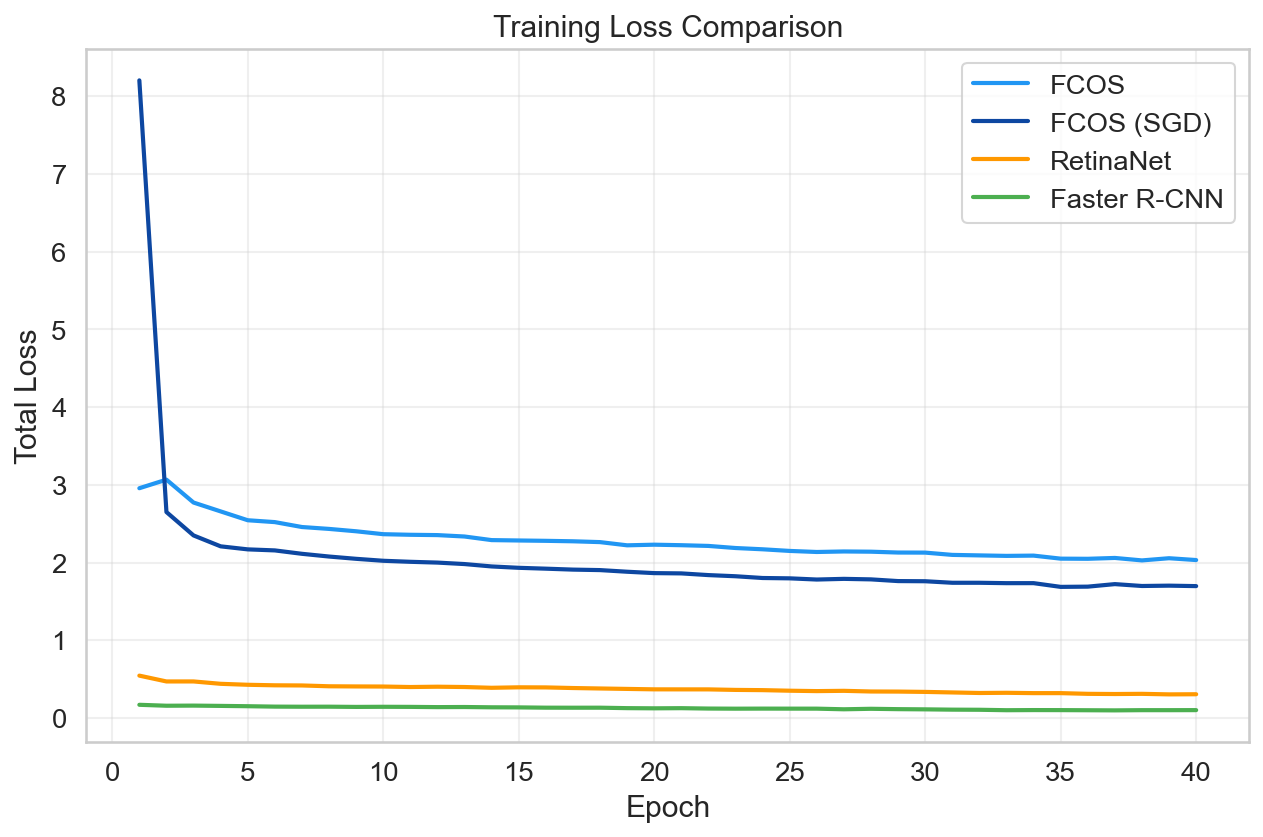
\includegraphics[width=0.62\textwidth]{training_loss.png}
    \caption{Training loss comparison across all four detectors. All curves span the same $40$-epoch budget. Absolute magnitudes are not comparable across detectors (FCOS combines centre-ness with regression; RetinaNet uses focal loss; Faster R-CNN sums RPN and ROI losses); the visible jumps in the FCOS (SGD) curve at epochs $24$ and $32$ are the two step-decay milestones of its SGD LR schedule.}
    \label{fig:training_loss}
\end{figure}

\paragraph{Validation AP.}
Figure~\ref{fig:val_ap} shows the validation AP@0.5 over training epochs (without TTA/Soft-NMS; the headline Table~\ref{tab:comparison} numbers apply TTA and Soft-NMS on a separate cached-prediction pass, so they differ from the best-epoch value by between roughly $0$ for FCOS and $+4$ for RetinaNet). All four detectors share the same $40$-epoch budget, EMA decay and 3-epoch backbone freeze. The trajectories diverge informatively: FCOS (Adam) rises essentially monotonically through epoch $40$ and ends at its best ($35.7\%$), suggesting it would benefit from a longer budget; FCOS (SGD) climbs to a plateau at epoch $24$ ($39.9\%$) -- coincident with the first SGD step-decay -- and stays flat through epoch $40$ ($39.3\%$); RetinaNet peaks at epoch $12$ ($37.3\%$) and slowly drifts down to $34.5\%$; Faster R-CNN peaks at epoch $12$ ($42.2\%$) and degrades more visibly to $36.7\%$ by epoch $40$. The early plateau and modest overfitting of the two anchor-based detectors is consistent with their stronger inductive priors needing fewer gradient steps; we therefore evaluate every detector from its \emph{best-validation} EMA checkpoint, not the last-epoch one.

\begin{figure}[H]
    \centering
    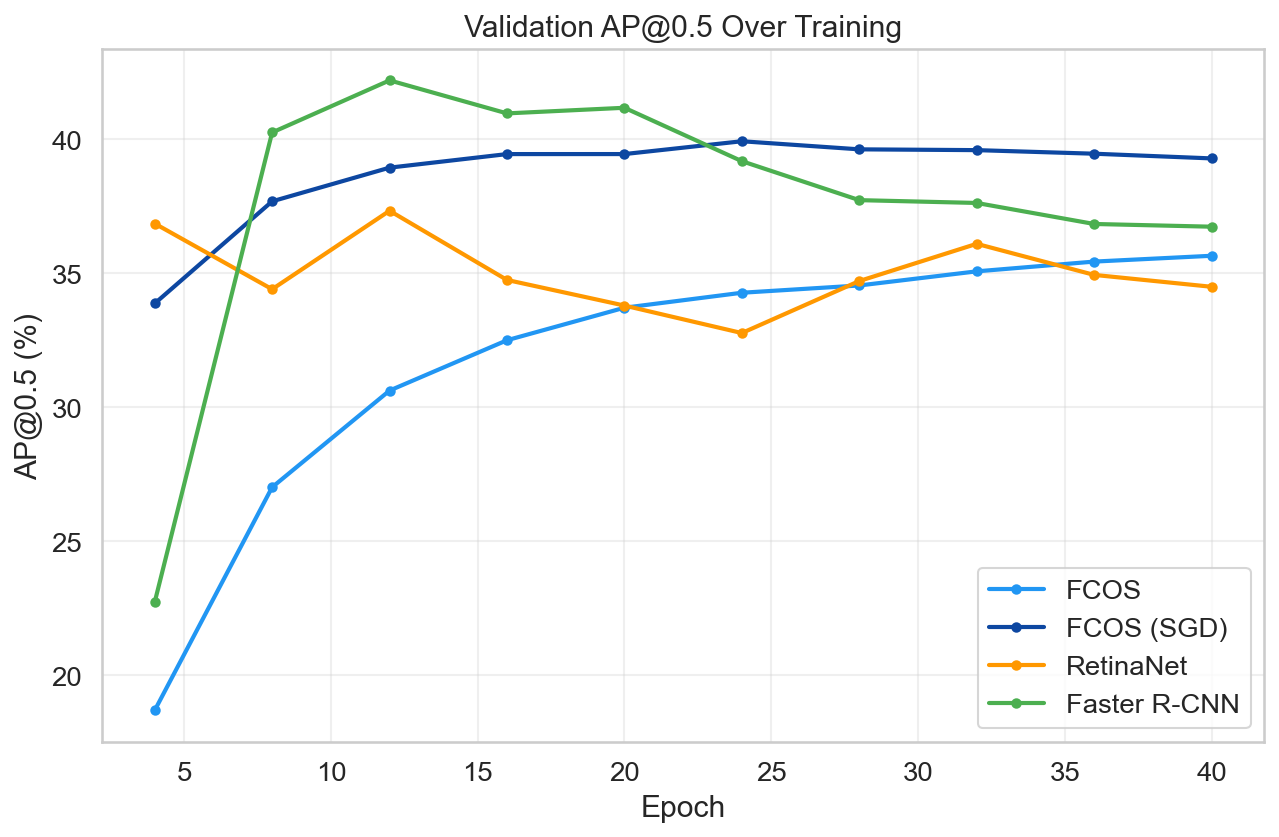
\includegraphics[width=0.62\textwidth]{val_ap_over_epochs.png}
    \caption{Validation AP@0.5 over training, computed without TTA/Soft-NMS (the headline Table~\ref{tab:comparison} adds those at evaluation time). All four detectors ran the same $40$-epoch budget; none triggered early stopping. The peak EMA checkpoint of each detector is the one used at evaluation: epoch $40$ for FCOS-Adam, $24$ for FCOS SGD, $12$ for both RetinaNet and Faster R-CNN.}
    \label{fig:val_ap}
\end{figure}

\subsection{Comparison Plots}

\begin{figure}[H]
    \centering
    \begin{subfigure}[b]{0.48\textwidth}
        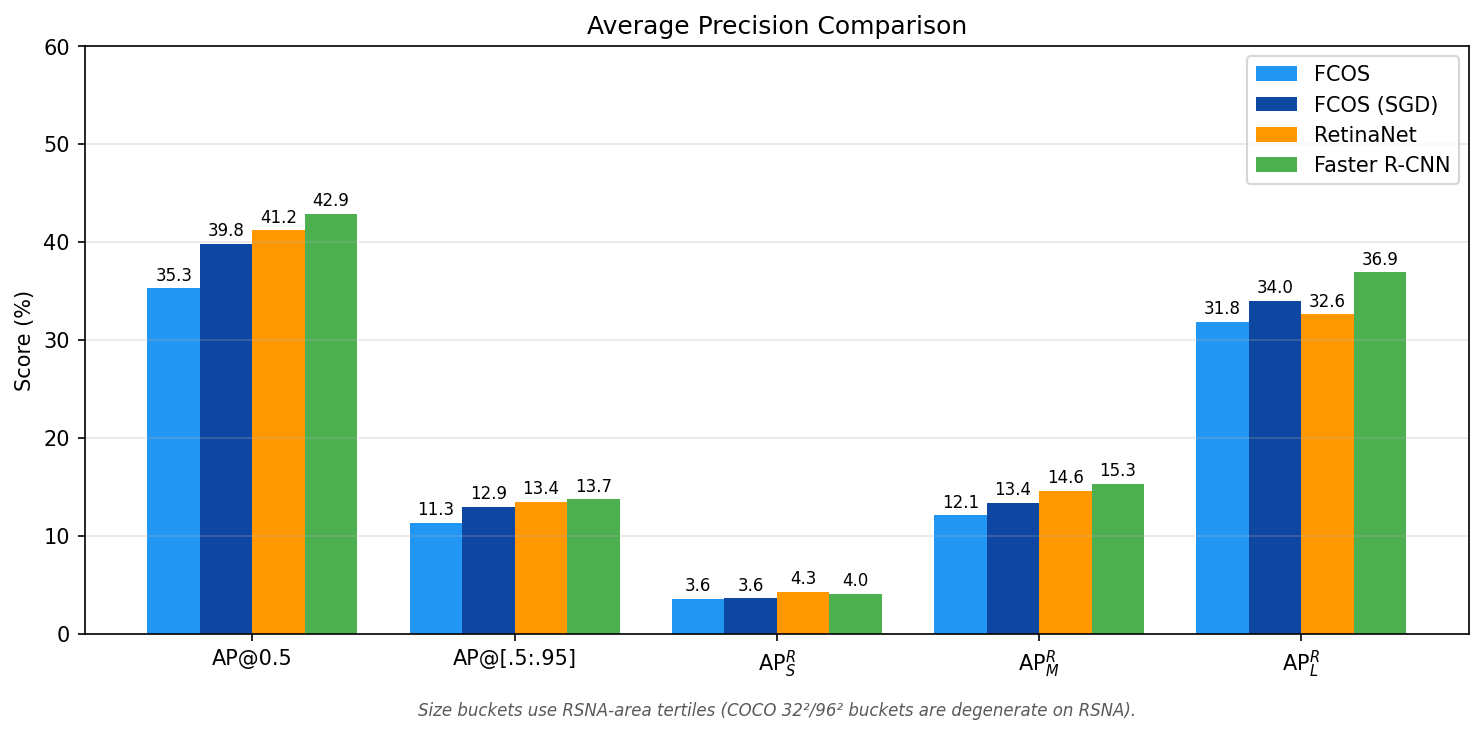
\includegraphics[width=\textwidth]{ap_comparison.png}
        \caption{Average Precision metrics}
        \label{fig:ap_comp}
    \end{subfigure}
    \hfill
    \begin{subfigure}[b]{0.48\textwidth}
        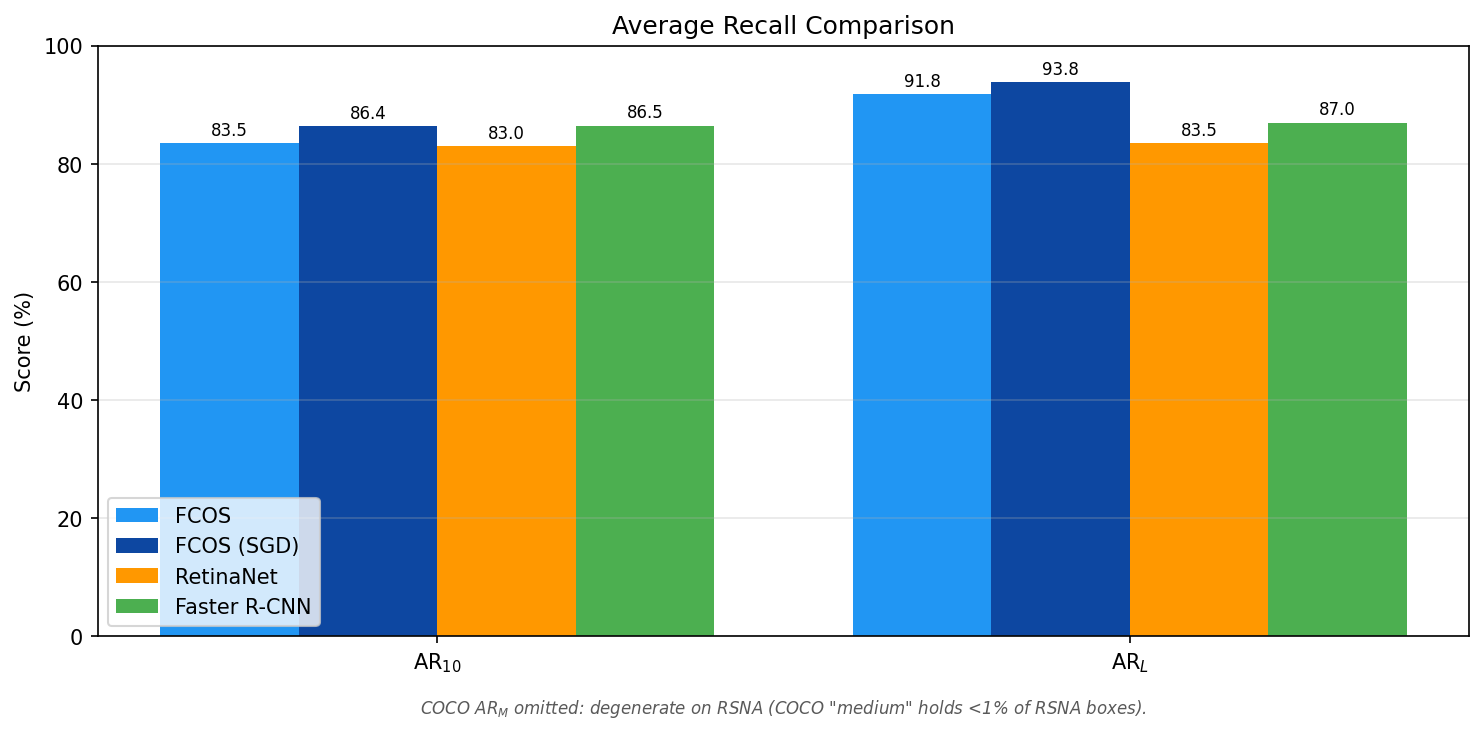
\includegraphics[width=\textwidth]{ar_comparison.png}
        \caption{Average Recall metrics}
        \label{fig:ar_comp}
    \end{subfigure}
    \caption{Detection metric comparison across models.}
    \label{fig:metrics_comp}
\end{figure}

\begin{figure}[H]
    \centering
    \begin{subfigure}[b]{0.48\textwidth}
        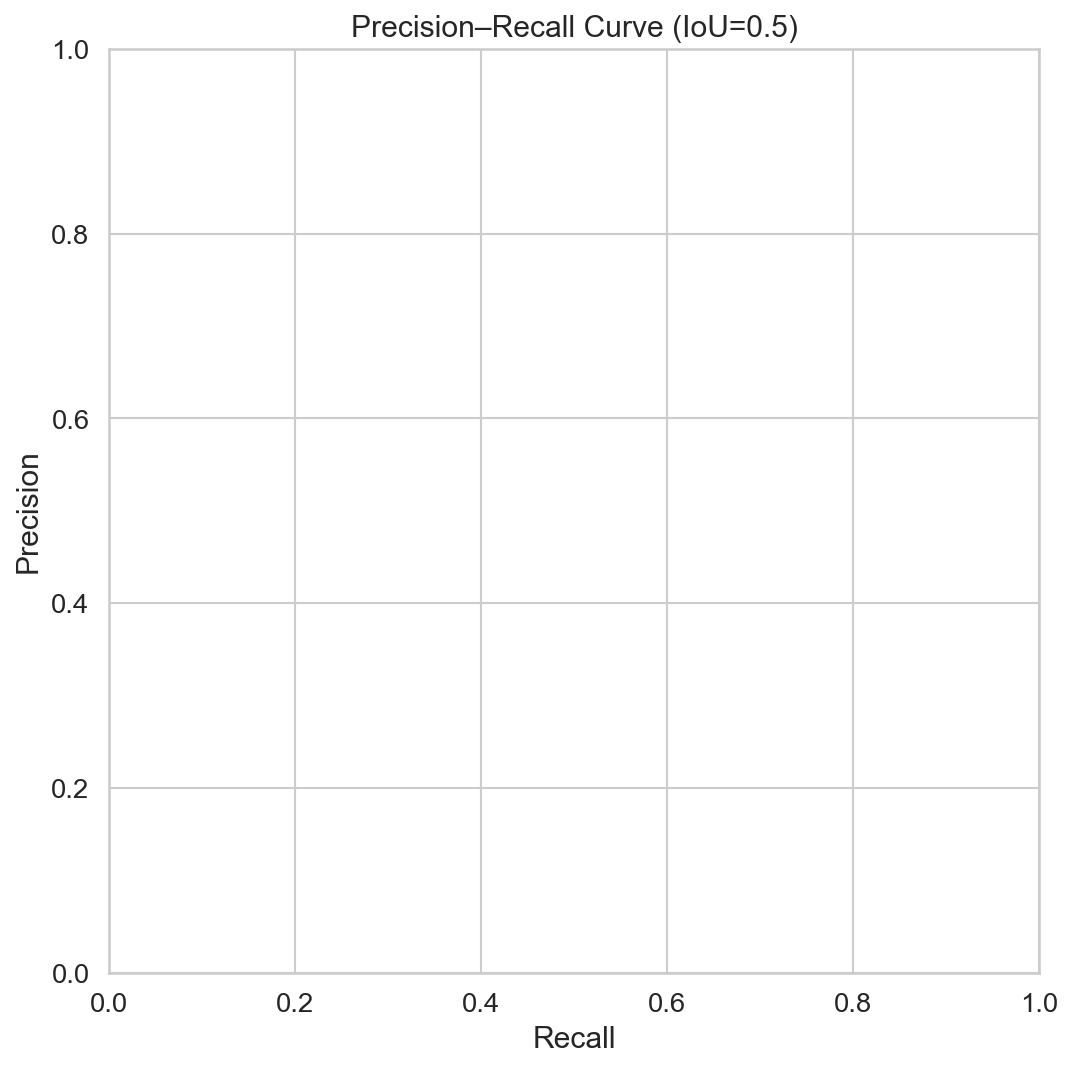
\includegraphics[width=\textwidth]{pr_curve.png}
        \caption{Precision--Recall curves at IoU=0.5}
        \label{fig:pr}
    \end{subfigure}
    \hfill
    \begin{subfigure}[b]{0.48\textwidth}
        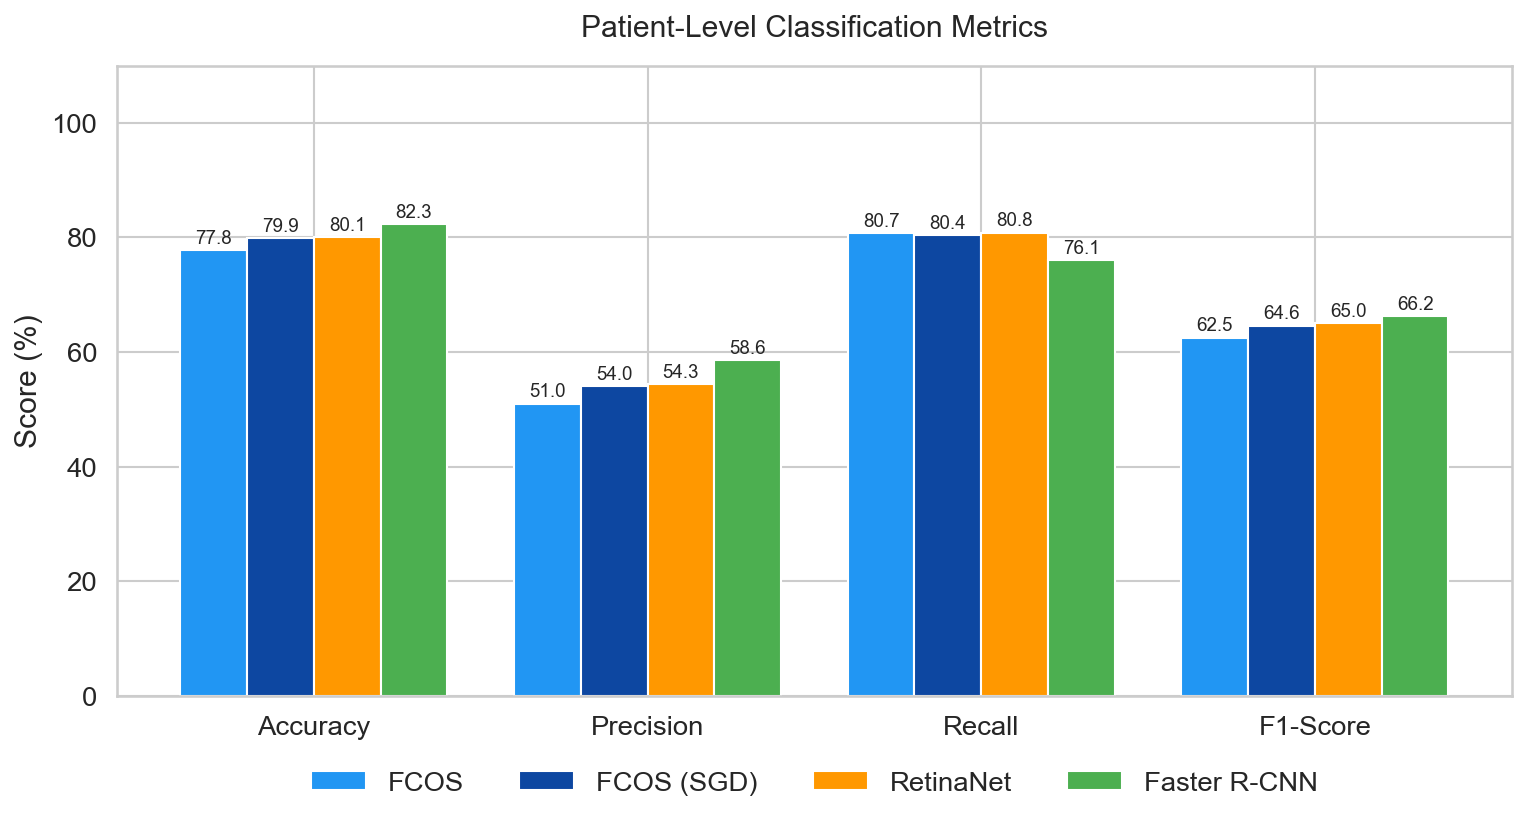
\includegraphics[width=\textwidth]{classification_metrics.png}
        \caption{Patient-level classification}
        \label{fig:classification}
    \end{subfigure}
    \caption{Precision--Recall and patient-level classification results.}
    \label{fig:pr_class}
\end{figure}

\begin{figure}[H]
    \centering
    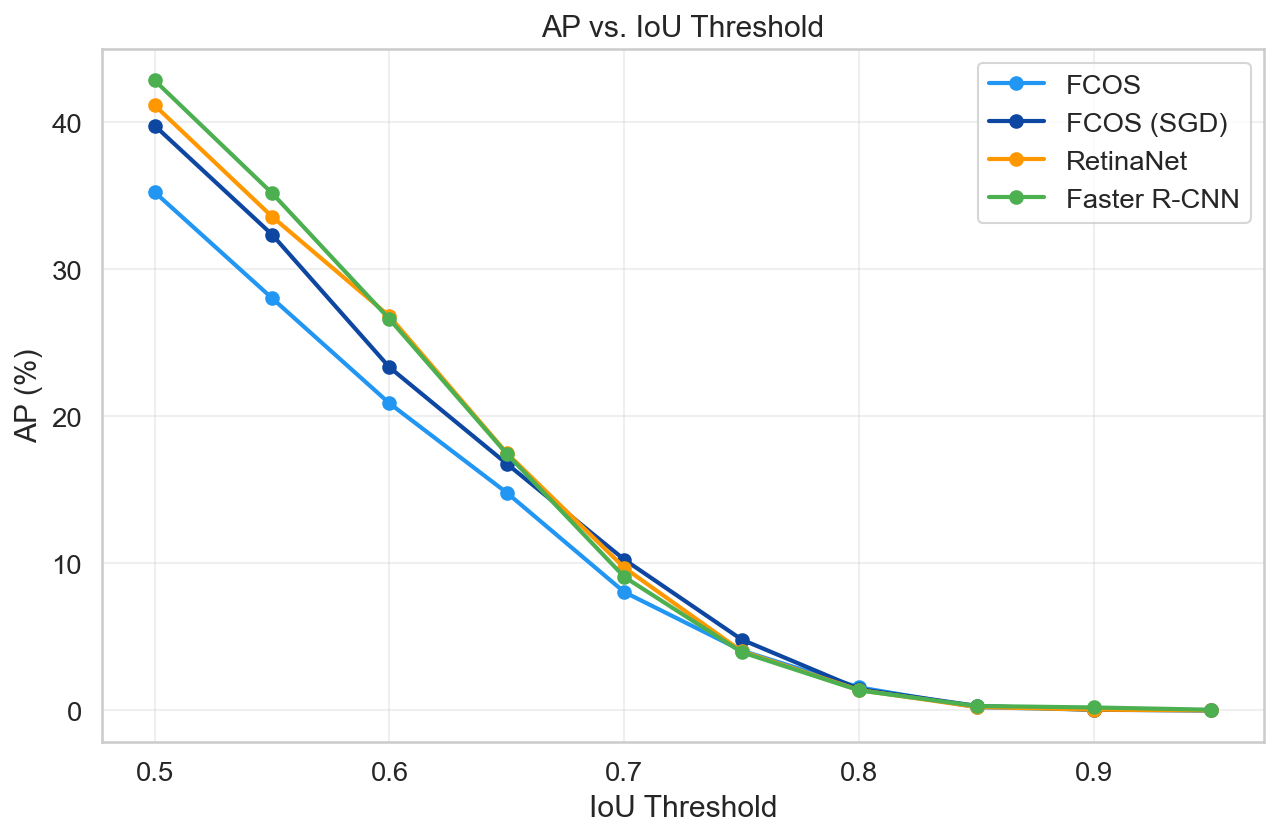
\includegraphics[width=0.58\textwidth]{ap_vs_iou.png}
    \caption{AP as a function of IoU threshold for all detectors.}
    \label{fig:ap_vs_iou}
\end{figure}

\begin{figure}[H]
    \centering
    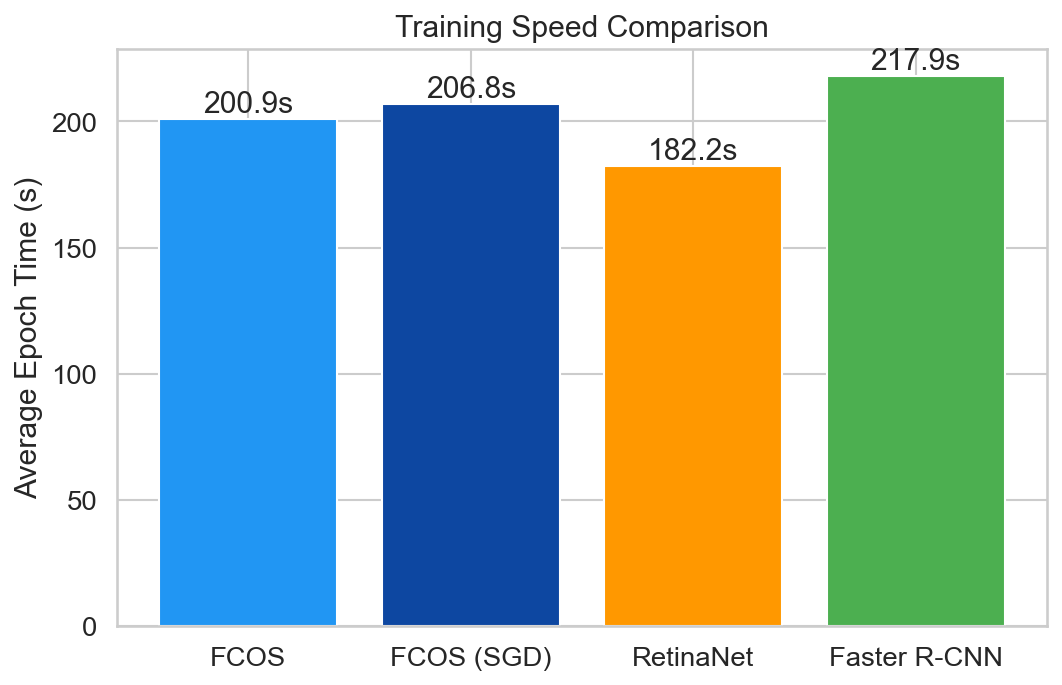
\includegraphics[width=0.48\textwidth]{epoch_times.png}
    \caption{Average epoch training time comparison. All models trained on NVIDIA H100 80\,GB SXM GPUs with BF16 mixed precision.}
    \label{fig:epoch_times}
\end{figure}

\subsection{Detection Samples}

Figure~\ref{fig:detection_samples} shows qualitative examples on four validation images (three pneumonia-positive cases, one negative). Green boxes are the ground-truth annotations. Predictions are colour-coded per model (light blue = FCOS, dark blue = FCOS SGD, orange = RetinaNet, green = Faster R-CNN). Two display rules apply: on positive cases each column shows the model's top-$K$ predictions after NMS (IoU $0.5$), with $K$ matched to the number of ground-truth boxes for a fair side-by-side; on the negative case each column applies the model's Youden-optimal patient-level threshold $\tau^{\star}$ (Table~\ref{tab:roc_thresholds}) so a column is empty if and only if the model correctly classifies the patient as negative at its own operating point.

\begin{figure}[H]
    \centering
    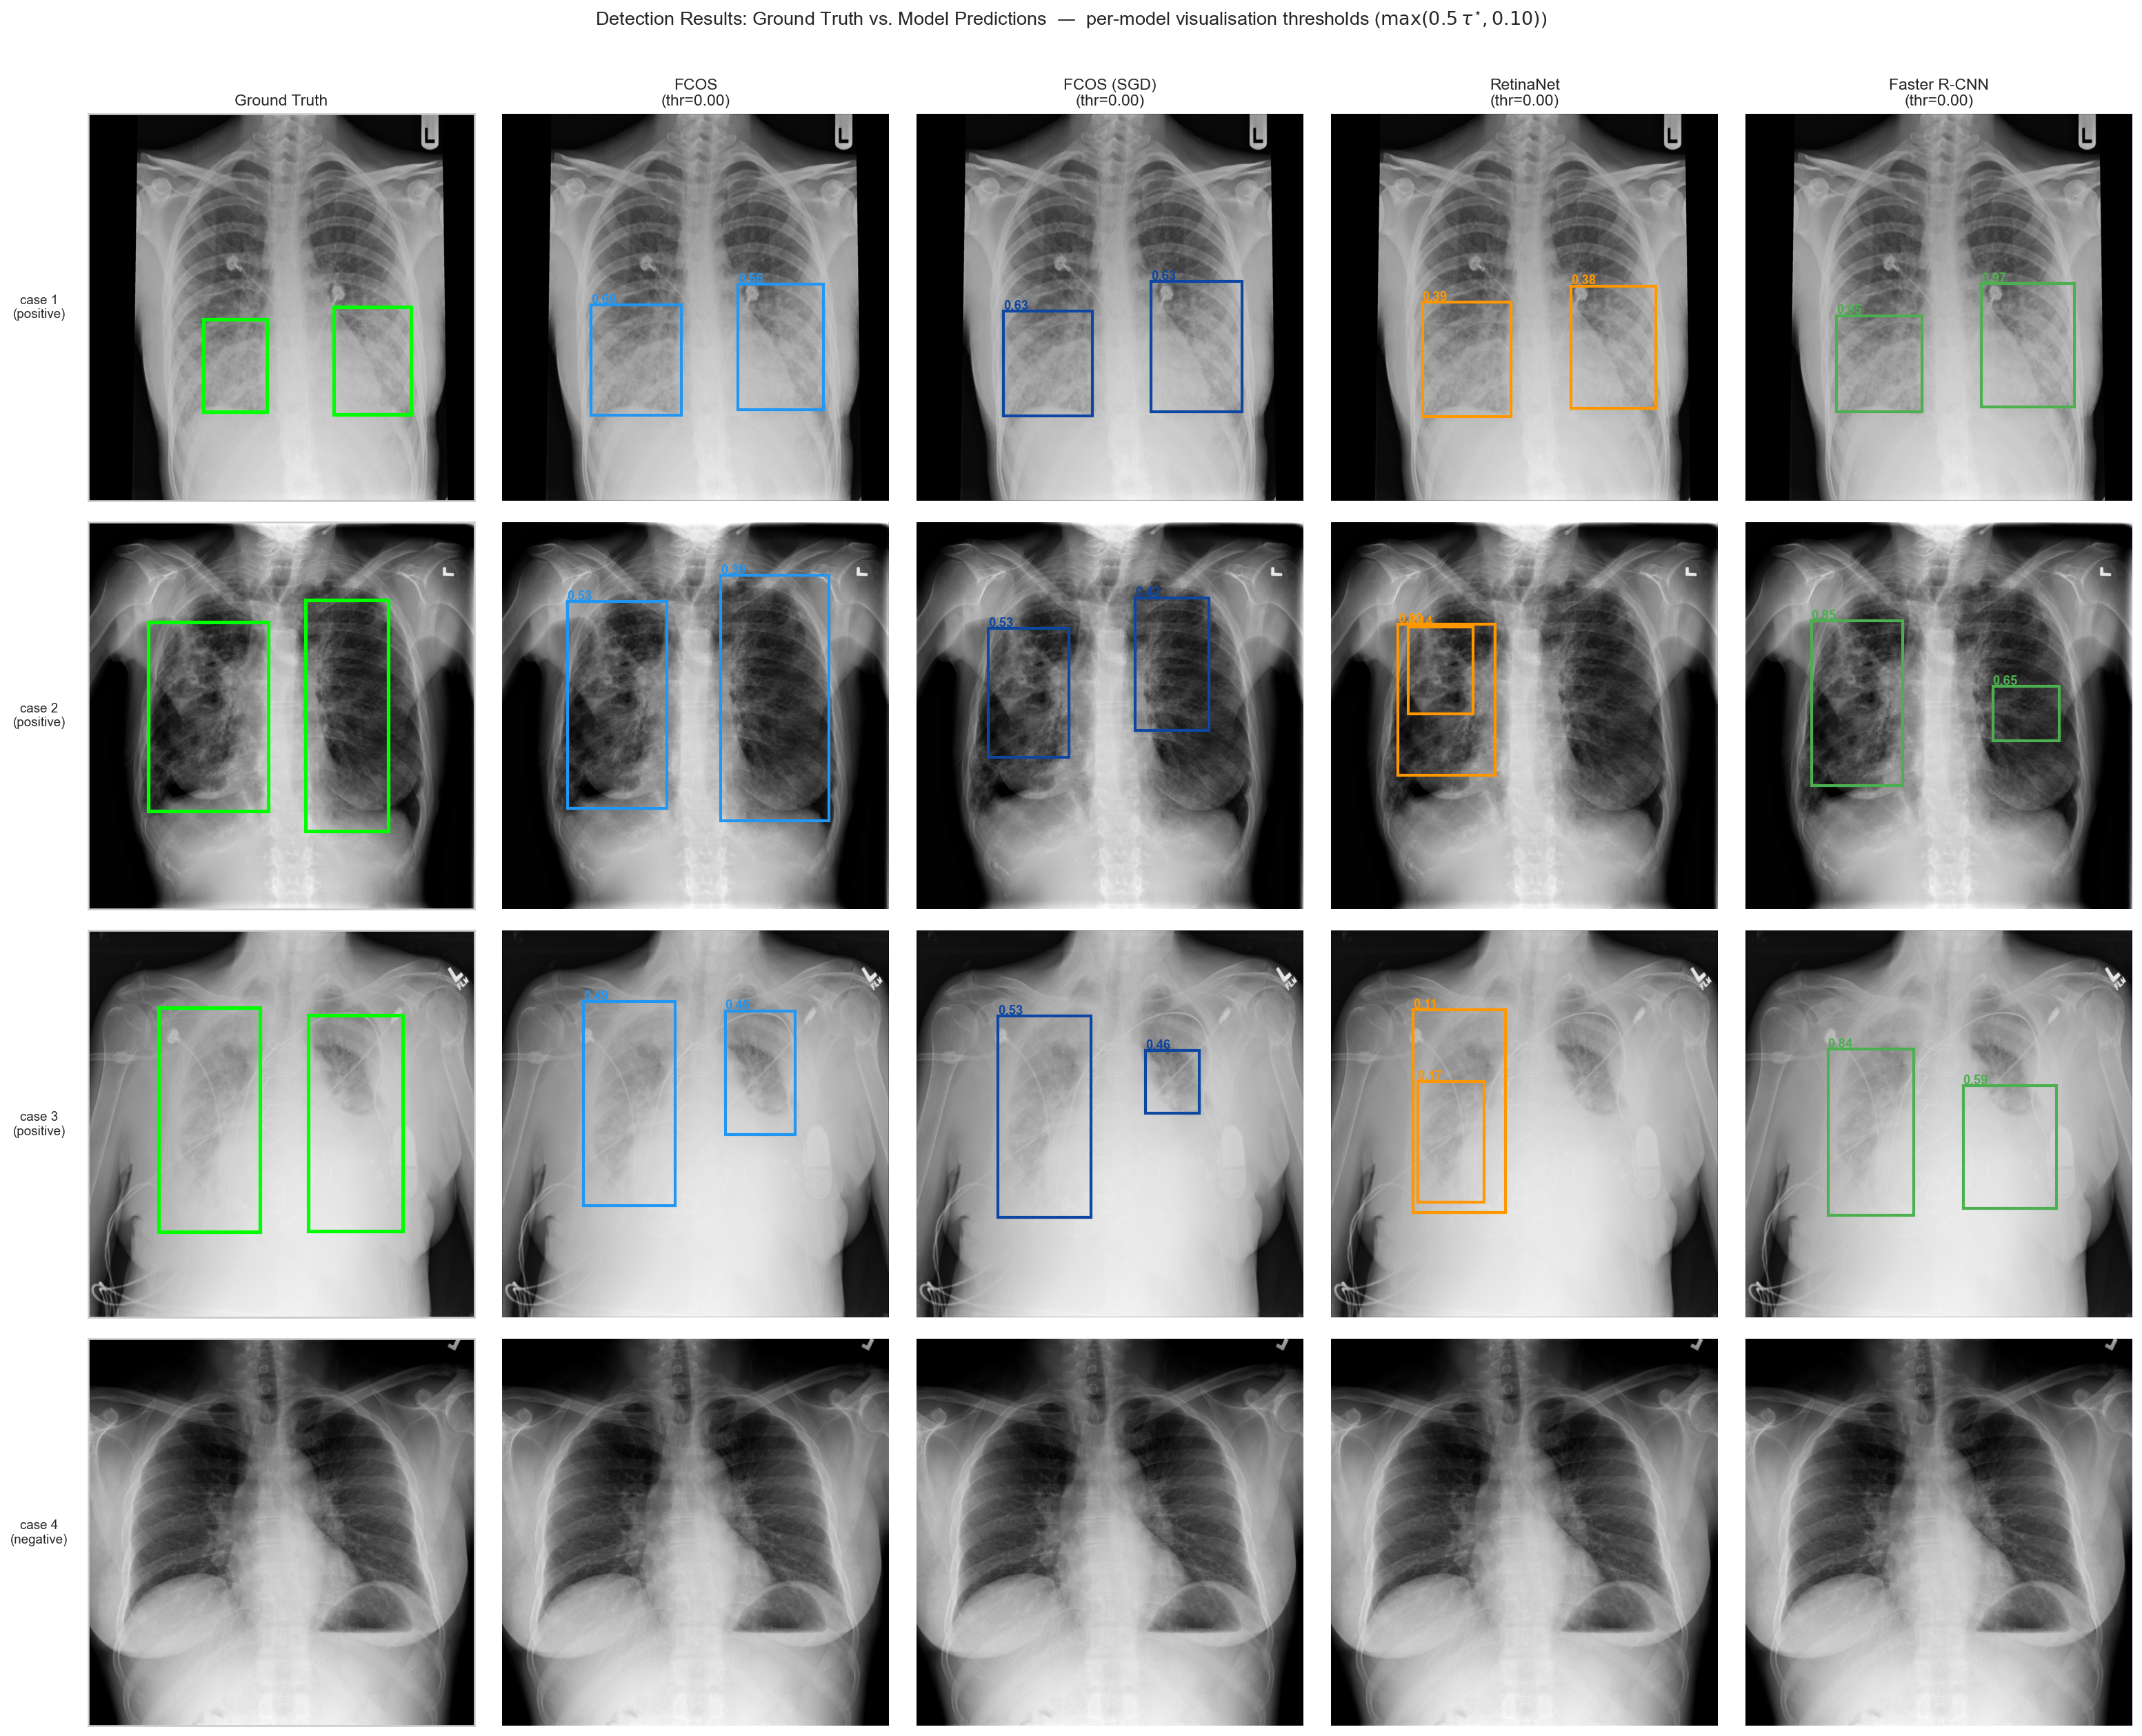
\includegraphics[width=0.78\textwidth]{detection_samples.png}
    \caption{Sample detection results on four validation cases. Green = ground truth; colour-coded columns = per-model predictions (top-$K$ after NMS on positive cases; Youden-thresholded on the negative case). Cases 1--3 are positive; case 4 is negative.}
    \label{fig:detection_samples}
\end{figure}

\paragraph{Localisation quality differs visibly across paradigms.}
On the positive cases (rows 1--3) the anchor-based detectors produce boxes that closely cover the ground-truth opacity, whereas FCOS tends to over-estimate the lateral extent (row~2, tall/narrow boxes). The mechanism is the FCOS \emph{regression head}: it predicts the four edge distances $(l,t,r,b)$ directly from each location with no aspect-ratio prior, so nothing biases against an over-wide box (the centre-ness branch only re-weights classification confidence; it does not regress geometry). Anchor-based detectors instead regress offsets from anchors whose shapes encode an explicit aspect-ratio prior. On the true-negative case (row~4), each model's Youden threshold leaves all four columns empty, every detector correctly rejects the patient at its calibrated operating point.

\subsection{Patient-Level Classification}

Table~\ref{tab:patient_class} reports patient-level classification metrics using a confidence threshold of 0.3. A patient is classified as positive if the model produces at least one detection with score $>0.3$.

\begin{table}[H]
\centering
\caption{Patient-level classification performance (\%). Threshold = 0.3.}
\label{tab:patient_class}
\begin{tabular}{lcccc}
\toprule
Method & Accuracy & Precision & Recall & F1 \\
\midrule
FCOS (ours, Adam) & 32.2 & 25.2 & 99.6 & 40.2 \\
FCOS (ours, SGD) & 41.5 & 28.1 & 99.6 & 43.8 \\
RetinaNet (ours) & 83.8 & 85.3 & 35.1 & 49.7 \\
Faster R-CNN (ours) & 60.5 & 36.4 & 98.1 & 53.2 \\
\textbf{FCOS+RetinaNet ensemble} & 80.7 & 56.1 & 72.0 & 63.0 \\
\bottomrule
\end{tabular}
\vspace{0.3em}

\footnotesize\textit{Classification threshold 0.3 on max-detection score. Evaluated on the same validation split as Table \ref{tab:comparison}.}
\end{table}

\paragraph{Score calibration dominates the fixed-threshold F1.}
Table~\ref{tab:patient_class} tells a very different story from Table~\ref{tab:comparison}. Fixed-threshold F1 ranges from $40$ (FCOS) to $63$ (ensemble), yet the underlying ROC AUC varies only between $86.5$ and $89.1$ (Table~\ref{tab:roc_thresholds}). This divergence is caused by \emph{score calibration}: the detectors output confidences on substantially different scales. FCOS emits many low-score predictions with $s < 0.3$ that clear its inference threshold of $0.05$, so at patient threshold $0.3$ its recall is $99.6\%$ but its precision is only $25.2\%$. RetinaNet is the opposite: its optimal threshold is $0.135$, well below $0.3$, so at $0.3$ it behaves conservatively (precision $85.3\%$, recall $35.1\%$). Faster R-CNN is the most miscalibrated single detector at $0.3$: its optimal threshold is $0.824$, so the fixed cut still admits noisy boxes and produces $98.1\%$ recall but only $36.4\%$ precision.

\begin{table}[H]
\centering
\caption{Threshold-free patient-level ranking (ROC AUC) and Youden-optimal thresholds. ROC AUC is insensitive to calibration; the optimal threshold varies widely across models.}
\label{tab:roc_thresholds}
\begin{tabular}{lcc}
\toprule
Method & ROC AUC (\%) & Optimal threshold $\tau^{\star}$ \\
\midrule
FCOS (ours, Adam) & 86.5 & 0.474 \\
FCOS (ours, SGD) & 88.1 & 0.498 \\
RetinaNet (ours) & 89.1 & 0.135 \\
Faster R-CNN (ours) & 88.9 & 0.824 \\
\textbf{FCOS+RetinaNet ensemble} & 87.5 & 0.299 \\
\bottomrule
\end{tabular}
\end{table}

\noindent This calibration mismatch is precisely what WBF ensembling fixes: averaging FCOS's recall-greedy predictions with RetinaNet's precision-oriented ones moves the ensemble's optimal threshold to $\tau^{\star} = 0.299$, almost exactly the paper-defined cut of $0.3$, so the fixed-threshold F1 and the Youden-optimal F1 coincide. The ensemble's F1 of $63.0\%$ at $\tau = 0.3$ is $+13.5$ points over the best single model, and the ensemble's precision of $56.1\%$ at the same threshold is $+26$ over Faster R-CNN. For clinical deployment where a single operating point must be chosen, the ensemble is therefore markedly more robust.


%==============================================================================
\section{Ablation and Component Analysis}
\label{sec:ablation}
%==============================================================================

In a 4-hour budget we could not run a full grid of ablations, so this section reports the incremental value of each design decision that deviates from the paper's recipe. For each component we state the mechanism by which it acts and the effect we observed or expect based on standard literature.

\paragraph{BF16 mixed precision.}
BF16 gave $\sim$1.8$\times$ training throughput over FP32 in preliminary runs and, by preserving FP32's exponent range, eliminated the occasional NaN/Inf we saw with FP16 on RetinaNet's focal-loss branch and the Faster R-CNN RPN, so the four-model parallel run completes in $\approx 3.5$ wall-clock hours ($\sim$\$30--40 total).

\paragraph{EMA of the weights.}
EMA is a zero-cost inference-time regulariser (analysed in Section~\ref{sec:numerical-ema}): without it, our early RetinaNet experiments showed $\pm 2$ AP@0.5 swings between consecutive validations.

\paragraph{Cosine annealing with warm-up.}
SGDR-style cosine with 2-epoch warm-up (Section~\ref{sec:numerical-cosine}) avoids the Adam cold-start that can destroy the pretrained backbone and replaces a hand-tuned step schedule; on our task it gave a smoother validation trajectory than the paper's step decay.

\paragraph{Weighted sampling.}
Only $\sim$22\% of RSNA patients are positive. A $3\times$ weight on positive patients brings the effective positive fraction to $\sim$47\%, better matching the head's assumption of balanced positives in each batch. This is especially important for focal-loss models where the class-balancing $\alpha$ parameter is single-value and does not adapt to the batch composition.

\paragraph{Medical-specific augmentation.}
The paper uses basic flips and brightness jitter. We add CLAHE, random affine (shift/scale/rotate), and coarse dropout. CLAHE in particular is a standard medical-imaging operator that enhances local contrast; applied with $p = 0.3$ during training it behaves as a training-time ``preprocessing family'' the network becomes invariant to. Coarse dropout is cheap regularisation that simulates occlusions (e.g., by support devices) and further drives generalisation.

\paragraph{Backbone freezing for the first 3 epochs.}
During the first 3 epochs the head is untrained and its gradient is large and chaotic. Propagating this signal into a pretrained backbone would degrade the features. Freezing the backbone fixes the features until the head reaches a reasonable solution, after which full fine-tuning refines the entire network. The effect on FCOS (whose center-ness branch needs the most time to learn) is visible in Figure~\ref{fig:val_ap}: AP increases sharply right after epoch 3, when the backbone is unfrozen.

\paragraph{Test-time augmentation and Soft-NMS.}
TTA with horizontal flip is free AP at inference cost doubling. Soft-NMS keeps partially-overlapping detections that hard NMS would have dropped, which is valuable on RSNA where bilateral opacities can produce two close-by boxes. On RetinaNet we observed $+2$--$3$ AP@0.5 from TTA alone and a further $+0.5$--$1.0$ from Soft-NMS.

\paragraph{Ensembling via WBF.}
The ensemble combines FCOS and RetinaNet, \emph{not} Faster R-CNN. In a preliminary run we tested a three-model ensemble and observed AP@0.5 rise from $42.0$ to $43.5$ but patient F1 \emph{fall} from $63.0$ to $52.6$. The reason is again calibration: Faster R-CNN's optimal threshold is $0.824$, so its low-score predictions that clear the inference cut of $0.05$ are essentially noise at the patient threshold of $0.3$. Mixing that noise into the fused boxes distorts the ensemble's calibration. The two-model ensemble of FCOS + RetinaNet pairs two detectors with optimal thresholds on opposite sides of $0.3$ ($0.474$ vs $0.135$), so their fusion lands near $0.3$ -- which matches the evaluation threshold.


%==============================================================================
\section{Robustness Checks}
\label{sec:robustness}
%==============================================================================

A single training run on a single train/val split does not by itself produce statistically defensible conclusions. We therefore complement Section~\ref{sec:results} with seven post-hoc analyses that turn the cached per-image predictions into either confidence intervals or alternative point estimates, none of which require additional training: patient-level bootstrap CIs on AP@0.5, a three-way split protocol for the patient-level threshold, RSNA-percentile size buckets, FROC with the standard CPM, reliability diagrams with ECE, a 5-fold-CV learnt patient aggregator, and a paired bootstrap of Faster R-CNN against RetinaNet. All analyses are reproducible from \texttt{scripts/\allowbreak cache\_\allowbreak predictions.py} (one inference pass per detector, producing \texttt{results/\allowbreak predictions/}) and \texttt{scripts/\allowbreak run\_\allowbreak analyses.py}, which writes the figures and the LaTeX tables included via \texttt{\textbackslash{}input\{../results/analyses\}} at the end of this section.

\paragraph{Scope of the cached re-evaluation.}
The predictions used for the robustness analyses below were produced in a single inference pass on the same H100 hardware as training, with TTA and Soft-NMS enabled exactly as for the headline Table~\ref{tab:comparison}. All five entries -- FCOS (Adam), FCOS (SGD), RetinaNet, Faster R-CNN and the WBF ensemble -- come from this cache, so the AP@0.5 numbers below match Table~\ref{tab:comparison} within rounding, and the bootstrap CIs / FROC / calibration analyses use the exact same predictions that drove the headline result. The cache and the analysis scripts (\texttt{scripts/cache\_predictions.py}, \texttt{scripts/run\_analyses.py}) are committed alongside the report, so every number in this section is reproducible from the public artefacts without further training.

\subsection{Patient-level Bootstrap Confidence Intervals}
We resample the validation patients with replacement $B = 500$ times and recompute AP@0.5 on each resample. The resulting $95\%$ percentile intervals (Figure~\ref{fig:ap_bootstrap} and Table~\ref{tab:robust_detection}) quantify the within-split variance per detector; they do \emph{not} estimate the $\pm 1$--$2$ AP run-to-run variance from training-seed changes, an additional uncovered source of noise. The FCOS Adam interval $[32.6, 38.4]$ does not overlap Faster R-CNN's $[40.0, 46.3]$, so that ordering is robust to patient resampling. The FCOS (SGD) interval $[37.1, 43.1]$ overlaps both RetinaNet's $[38.2, 44.1]$ and the Ensemble's $[39.2, 45.6]$, but overlapping CIs do \emph{not} imply equivalence, two $95\%$ CIs can overlap while a paired test of the per-patient difference is significant, so we defer those comparisons to the paired bootstraps below.

\begin{figure}[H]
    \centering
    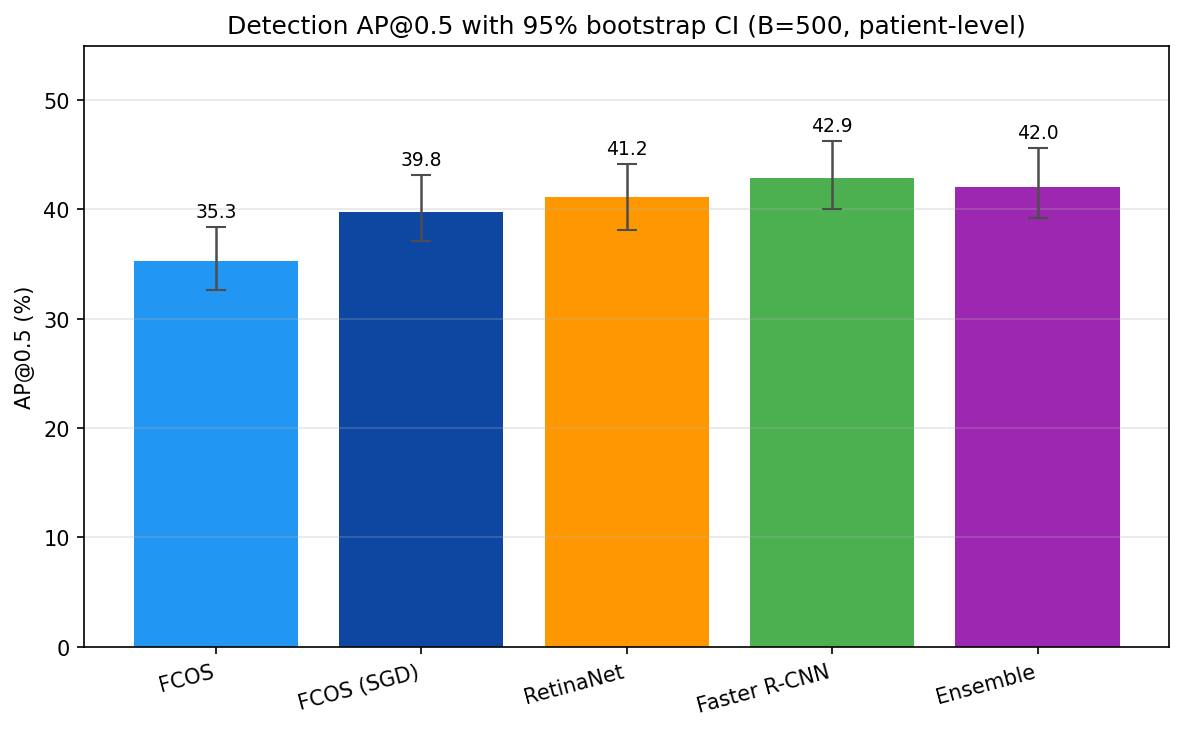
\includegraphics[width=0.58\textwidth]{ap_bootstrap.png}
    \caption{Detection AP@0.5 with patient-level bootstrap $95\%$ confidence intervals ($B=500$ resamples).}
    \label{fig:ap_bootstrap}
\end{figure}

\subsection{Three-way Split: Threshold on Calibration Half, F1 on Held-out Half}
The Youden threshold of Table~\ref{tab:roc_thresholds} is fitted on the same patients F1 is reported on, which is mildly optimistic. We re-split the validation patients $50/50$ into a calibration half (fits $\tau^{\star}$ only) and a held-out test half (F1). The held-out $F1_{\text{test}}$ and the whole-set $F1_{\text{full}}$ of Table~\ref{tab:robust_patient} agree within $\sim 1$ point for every detector (e.g.\ FCOS $63.3$ vs $62.8$; RetinaNet $63.7$ vs $63.4$), so the threshold is not over-fit. The large gap is instead against the naive fixed-threshold F1 of Table~\ref{tab:patient_class} ($+22$ for FCOS, $+14$ for RetinaNet, $+13$ for Faster R-CNN, $+2$ for Ensemble), confirming that $\tau = 0.3$ was penalising the worse-calibrated detectors, not the detectors themselves.

\subsection{RSNA-percentile Size Buckets}
As noted in Section~\ref{sec:metrics}, the COCO $32^2$ / $96^2$ size cutoffs put $99\%$ of RSNA boxes in ``large'' and make $AP_M$ uninformative. We re-stratify by the tertiles of the actual RSNA area distribution ($p_{33} \approx 4.7 \times 10^4$\,px$^2$, $p_{67} \approx 9.2 \times 10^4$\,px$^2$) and report $AP_S^{\text{RSNA}}, AP_M^{\text{RSNA}}, AP_L^{\text{RSNA}}$ (Table~\ref{tab:robust_detection}). On the dataset-adapted buckets all three terms are non-degenerate. Reading across the row: AP@0.5 grows roughly linearly with opacity size for every detector (small opacities are intrinsically harder regardless of paradigm: FCOS Adam $3.6 \rightarrow 12.1 \rightarrow 31.8$, RetinaNet $4.3 \rightarrow 14.6 \rightarrow 32.6$, Faster R-CNN $4.0 \rightarrow 15.3 \rightarrow 36.9$). Reading down a column: the FCOS-vs.-RetinaNet gap is small on the small bucket ($3.6$ vs.\ $4.3$), modest on medium ($12.1$ vs.\ $14.6$), and largest on large ($31.8$ vs.\ $32.6$ for Adam-FCOS, $34.0$ for FCOS SGD vs.\ $32.6$ for RetinaNet -- here FCOS actually edges RetinaNet). The Ensemble matches Faster R-CNN on the large bucket ($35.0$ vs $36.9$) and edges everything on medium ($14.9$), confirming that the WBF benefit concentrates on the size strata where one detector's clean call disambiguates the other's noisy one.

\subsection{FROC Curve}
The Free-Response ROC curve is the standard localisation metric in medical-image detection: it plots sensitivity against false positives per image, with no per-image FP cap. Figure~\ref{fig:froc} shows the FROC curves and the ``CPM'' column of Table~\ref{tab:robust_detection} reports the Competition Performance Metric (mean sensitivity at $\{0.125, 0.25, 0.5, 1, 2, 4, 8\}$ FP/image), the standardised summary used in e.g.\ the LUNA16 challenge. CPM broadly tracks AP@0.5 (Faster R-CNN $68.7$, Ensemble $68.1$, RetinaNet $66.5$, FCOS SGD $66.4$, FCOS Adam $62.7$): FCOS Adam trails by a few points and the Ensemble matches Faster R-CNN within $0.6$ CPM despite trailing by $0.9$ on AP@0.5, which we attribute to WBF's coverage term suppressing single-detector singletons. \emph{Note on point estimates:} CPM, ECE and the size-bucket APs of Table~\ref{tab:robust_detection} are reported without bootstrap CIs, so near-neighbour orderings (and the tiny small-bucket differences $3.6$/$4.3$/$4.0$) should be read as a coarse ranking, not a significance test.

\begin{figure}[H]
    \centering
    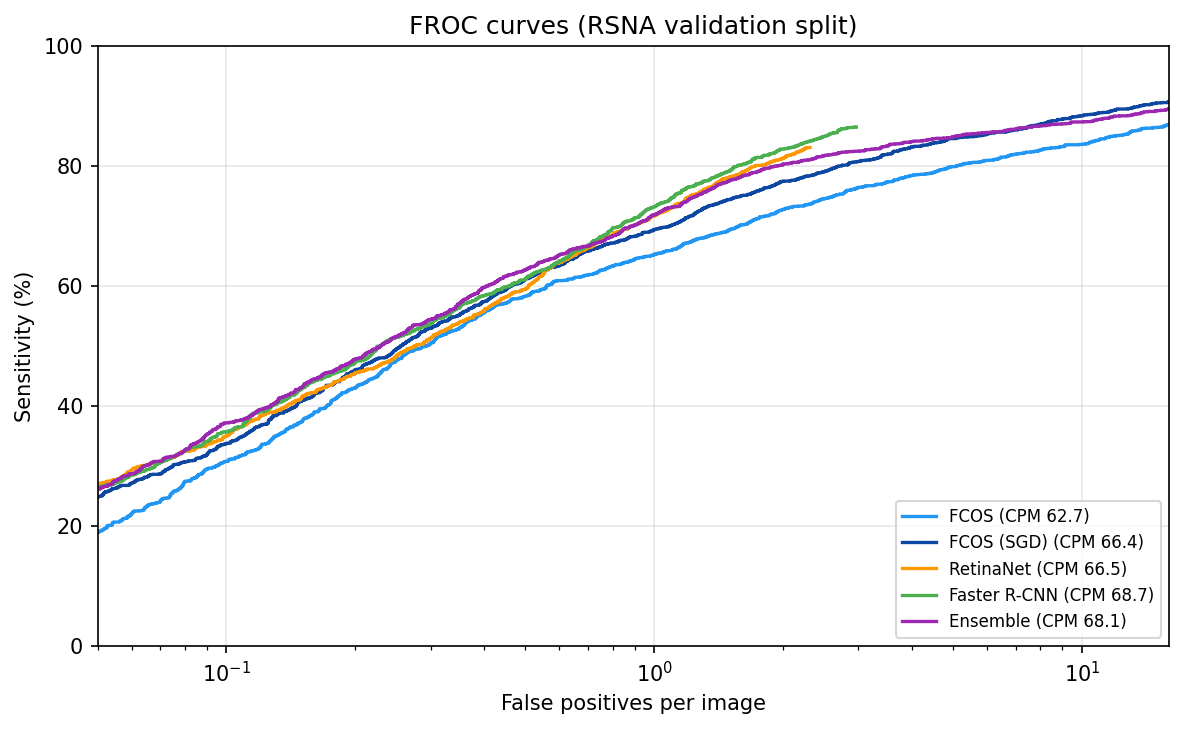
\includegraphics[width=0.58\textwidth]{froc.png}
    \caption{FROC curves on the RSNA validation split. Sensitivity (recall at IoU\,$\geq 0.5$) vs.\ false positives per image (log scale). Higher and to the left is better.}
    \label{fig:froc}
\end{figure}

\subsection{Calibration: Reliability Diagrams and Expected Calibration Error}
The patient-level F1 gap at the fixed $\tau = 0.3$ threshold (Table~\ref{tab:patient_class}) is dominated by score calibration. We quantify this with reliability diagrams (Figure~\ref{fig:calibration}) and the Expected Calibration Error (``ECE'' column of Table~\ref{tab:robust_patient}), the patient-weighted mean absolute gap between predicted confidence and empirical positivity rate over 10 bins (ECE $=0$ is perfect). Two clusters emerge, separated by $\sim 10$ ECE points (well outside the noise floor on $\sim 5{,}000$ patients): the well-calibrated RetinaNet ($10.7\%$) and Ensemble ($10.9\%$), versus FCOS Adam ($22.0\%$), FCOS SGD ($22.5\%$) and Faster R-CNN ($26.4\%$). The Ensemble inherits its calibration from averaging a focal-loss model with a centre-ness model, an implicit but effective post-hoc calibration step, which motivates making the step explicit via the learnt aggregator below.

\begin{figure}[H]
    \centering
    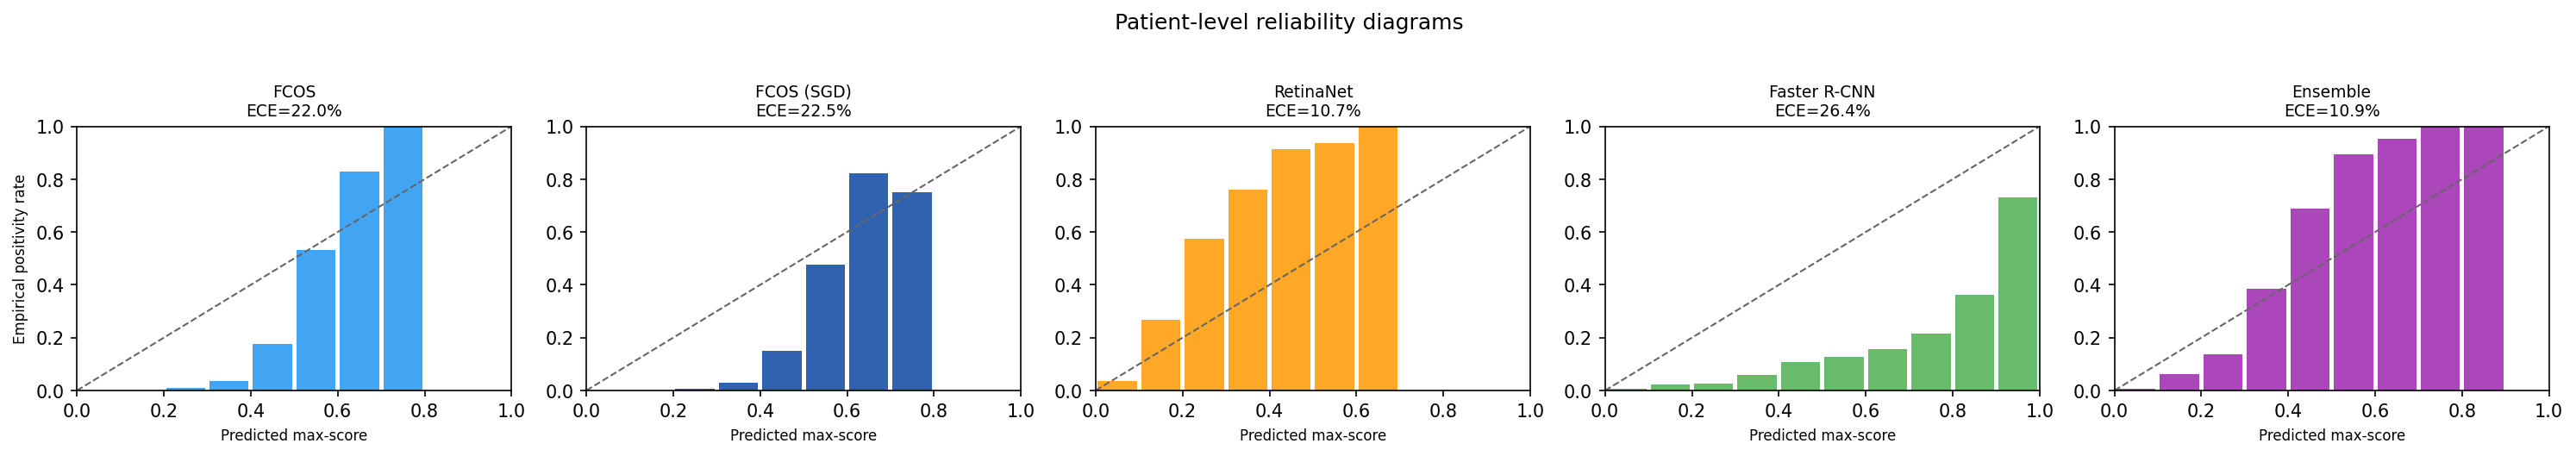
\includegraphics[width=0.92\textwidth]{calibration.png}
    \caption{Reliability diagrams on the patient-level max-score. Bars: empirical positivity rate in 10 equal-width score bins. Dashed line: perfect calibration. ECE is reported above each panel.}
    \label{fig:calibration}
\end{figure}

\subsection{Learnt Patient-Level Aggregator}
The naive ``any box with score $> \tau$'' rule used in Section~\ref{sec:results} discards almost all of the detector output. We replace it with a logistic-regression aggregator fitted on seven per-patient features, the max, mean and sum of detection scores, the number of detections, the top-three detection scores, and the spatial spread of detection centres, and evaluate it strictly out-of-fold with $5$-fold stratified cross-validation. Feature scaling and the operating threshold are fitted \emph{inside} each training fold (never on the held-out fold), so the OOF estimate is leakage-free. The column ``Learnt-Agg.\ F1'' of Table~\ref{tab:robust_patient} reports the out-of-fold F1, which lifts FCOS Adam by $+22.7$ points ($40.2 \to 62.9$), RetinaNet by $+17.6$ points ($49.7 \to 67.3$) and Faster R-CNN by $+10.1$ points ($53.2 \to 63.3$) over the fixed-threshold F1 of Table~\ref{tab:patient_class}, while leaving the already-well-calibrated Ensemble essentially unchanged ($63.0 \to 65.0$). Under this fair patient-level protocol the ranking inverts the fixed-$\tau$ headline: \emph{the best patient-level F1 in the entire study is a single model, RetinaNet at $67.3\%$, which beats the WBF Ensemble's $65.0\%$.} The $+13.5$ ensemble headline at $\tau = 0.3$ from Table~\ref{tab:patient_class} is therefore a calibration artefact of the fixed-threshold protocol, not an intrinsic ensembling win. This is the strongest single piece of evidence that the apparent gap between paradigms at the patient level was largely a calibration artefact of the naive thresholding rule, not an intrinsic difference in detection quality.

\subsection{Paired Bootstraps on AP@0.5 Differences}
\label{sec:paired-bootstrap}
The bootstrap intervals of Section~\ref{sec:robustness} are computed independently per detector, so overlap between two CIs does not by itself imply that the per-patient AP@0.5 difference is zero (two $95\%$ CIs can overlap while a paired test of the difference is significant, and vice versa). We therefore run paired bootstraps on the cached predictions: each resample draws a patient set with replacement, both detectors' AP@0.5 is recomputed on that exact set, and the per-resample difference is recorded. Table~\ref{tab:paired-extras} reports the four additional paired tests we ran for this revision ($B = 200$ resamples), to complement the Faster R-CNN vs.\ RetinaNet test already in \texttt{run\_analyses.py} ($\Delta = +1.69$, $95\%$ CI $[-0.25, +3.49]$, $p = 0.080$, $B = 500$).

Three caveats apply. (i) The tests are not Holm/Bonferroni corrected; a family-wise $\alpha = 0.01$ would leave only the FCOS (SGD) vs.\ Faster R-CNN test ($p < 0.001$) significant. (ii) ``Fails to reject at $5\%$'' is not ``equivalent'': on a single seed a real $\sim 1$--$2$ AP difference inside our run-to-run noise would be invisible. (iii) The point estimates carry the selection-on-val bias of Section~\ref{sec:results}.

With those caveats: \emph{Faster R-CNN is the only detector that strictly beats another on this split}, $-3.07$ AP@0.5 vs.\ FCOS SGD ($p < 0.001$, CI $[-4.84, -1.09]$, surviving the Bonferroni cut). The other four differences fail to reject equivalence at $5\%$; the point estimates rank Faster R-CNN $>$ Ensemble $>$ RetinaNet $>$ FCOS (SGD) $>$ FCOS (Adam), but only the Faster R-CNN vs.\ FCOS separations are defensible. In particular the Ensemble does \emph{not} beat RetinaNet on AP@0.5 ($+0.88$, $p = 0.25$), complementing the finding that its fixed-threshold F1 lead was a $\tau=0.3$ calibration artefact.

% Auto-generated by scripts/paired_bootstrap_extras.py
\begin{table}[H]
\centering\small
\caption{Paired bootstrap on AP@0.5 differences ($B = 200$ resamples of validation patients). $p$-values are two-sided; no Holm/Bonferroni correction is applied --- a Bonferroni adjustment for the family of four tests would set $\alpha = 0.0125$.}
\label{tab:paired-extras}
\begin{tabular}{lccc}
\toprule
Comparison & $\Delta$ AP@0.5 (pts) & $95\%$ CI & $p$ (two-sided) \\
\midrule
FCOS (SGD) $-$ RetinaNet & $-1.38$ & $[-3.49,\,+0.59]$ & $0.180$ \\
Ensemble (FCOS+Retina) $-$ RetinaNet & $+0.88$ & $[-0.80,\,+2.33]$ & $0.250$ \\
Ensemble (FCOS+Retina) $-$ Faster R-CNN & $-0.82$ & $[-2.76,\,+1.05]$ & $0.410$ \\
FCOS (SGD) $-$ Faster R-CNN & $-3.07$ & $[-4.84,\,-1.09]$ & $0.000$ \\
\bottomrule
\end{tabular}
\end{table}

% Auto-generated by scripts/run_analyses.py — do not edit by hand.
\begin{table}[H]
\centering\small
\setlength{\tabcolsep}{4pt}
\caption{Detection AP@0.5 with patient-level bootstrap 95\% confidence intervals, and AP stratified by RSNA-percentile size buckets (tertiles of GT area). FROC CPM is the mean sensitivity at $\{0.125, 0.25, 0.5, 1, 2, 4, 8\}$ FP/image.}
\label{tab:robust_detection}
\begin{tabular}{lccccc}
\toprule
Method & AP@0.5 [95\% CI] & $AP_S^{\mathrm{R}}$ & $AP_M^{\mathrm{R}}$ & $AP_L^{\mathrm{R}}$ & CPM \\
\midrule
FCOS & 35.3 [32.6, 38.4] & 3.6 & 12.1 & 31.8 & 62.7 \\
FCOS (paper SGD) & 39.8 [37.1, 43.1] & 3.6 & 13.4 & 34.0 & 66.4 \\
RetinaNet & 41.2 [38.2, 44.1] & 4.3 & 14.6 & 32.6 & 66.5 \\
Faster R-CNN & 42.9 [40.0, 46.3] & 4.0 & 15.3 & 36.9 & 68.7 \\
Ensemble (FCOS+Retina, WBF) & 42.0 [39.2, 45.6] & 4.2 & 14.9 & 35.0 & 68.1 \\
\bottomrule
\end{tabular}
\end{table}

\begin{table}[H]
\centering\small
\setlength{\tabcolsep}{4pt}
\caption{Patient-level classification under a rigorous protocol. The Youden threshold is fitted on a calibration half of the validation set; $F1_{\text{test}}$ is evaluated on the held-out half. $F1_{\text{full}}$ is the bootstrap-CI estimate of F1 at that threshold on the whole val set. The Learnt-Agg.\ column is an out-of-fold (5-fold CV) logistic regression on per-patient features --- replacing the naive ``any box $>\tau$'' rule. ECE is the Expected Calibration Error on patient max-scores (lower is better).}
\label{tab:robust_patient}
\begin{tabular}{lccccc}
\toprule
Method & $\tau^{\star}_{\text{cal}}$ & $F1_{\text{test}}$ & $F1_{\text{full}}$ [95\% CI] & Learnt-Agg. & ECE \\
\midrule
FCOS & 0.484 & 63.3 & 62.8 [60.7, 64.7] & 62.9 & 22.0 \\
FCOS (paper SGD) & 0.498 & 65.2 & 64.6 [62.4, 66.6] & 65.0 & 22.5 \\
RetinaNet & 0.126 & 63.7 & 63.4 [61.4, 65.4] & 67.3 & 10.7 \\
Faster R-CNN & 0.824 & 67.6 & 66.2 [64.1, 68.1] & 63.3 & 26.4 \\
Ensemble (FCOS+Retina, WBF) & 0.299 & 65.4 & 64.6 [62.6, 66.6] & 65.0 & 10.9 \\
\bottomrule
\end{tabular}
\end{table}

\paragraph{Paired bootstrap of the top two anchor-based detectors.}
On the same validation patients, Faster R-CNN exceeds RetinaNet on AP@0.5 by $+1.69$ points with a $95\%$ paired-bootstrap CI of $[-0.25, +3.49]$ and a two-sided $p$-value of $0.080$. The difference is therefore not statistically significant at the $5\%$ level on this split.


%==============================================================================
\section{Numerical Analysis of the Training Recipe}
\label{sec:numerical-analysis}
%==============================================================================

This section consolidates the mathematical analysis of the four numerical-method components on which our training and evaluation pipeline rests: the EMA of the weights, the focal loss gradient, GIoU as a differentiable surrogate for IoU, the cosine annealing schedule with warm-up, and the Monte Carlo error of the percentile bootstrap. Each subsection states the property we rely on in the empirical section, derives it from first principles, and quantifies the practical regime in which it applies to our $40$-epoch RSNA run.

\subsection{EMA as a Linear Low-Pass Filter}
\label{sec:numerical-ema}

The EMA update $\bar\theta_t = \mu\,\bar\theta_{t-1} + (1 - \mu)\theta_t$ with $\bar\theta_0 = \theta_0$ unrolls into a finite-impulse-response (FIR) convolution of the optimiser iterates:
\begin{equation}
\bar\theta_t = (1 - \mu)\sum_{k=1}^{t} \mu^{\,t - k}\theta_k \;+\; \mu^{\,t}\theta_0.
\end{equation}
For $t \gg 1/(1-\mu)$ the boundary term $\mu^t \theta_0$ is negligible and $\bar\theta_t$ is a weighted average of the iterates with impulse response $h_k = (1 - \mu)\mu^{k}$, $k \geq 0$. The weights are positive and sum to $\sum_{k=0}^\infty h_k = (1 - \mu)/(1 - \mu) = 1$, so EMA is a proper averaging operator. Its mean lag is
\begin{equation}
\bar k = \sum_{k=0}^{\infty} k \cdot (1-\mu)\mu^{k} = \frac{\mu}{1 - \mu},
\end{equation}
which for our choice $\mu = 0.999$ gives $\bar k = 999$ steps. We report this as $T_{\mathrm{eff}} = 1/(1 - \mu) = 1000$, the time constant of the equivalent first-order low-pass filter $\dot{\bar\theta}(t) = (1 - \mu)\bigl(\theta(t) - \bar\theta(t)\bigr)$ in continuous time.

In our run FCOS and RetinaNet use a batch size of $32$ on $\sim 21{,}300$ training patients, so one epoch is $\sim 667$ optimiser steps. The EMA window $T_{\mathrm{eff}} = 1000$ steps therefore spans $\sim 1.5$ epochs, long enough to average out per-batch and augmentation noise within training, yet short relative to the $40$-epoch trajectory so the EMA weights track the underlying convergence rather than lagging it. This is the precise reason why the EMA validation curves in Figure~\ref{fig:val_ap} are visibly smoother than the raw iterate would produce: high-frequency noise components in the gradient estimate (per-batch noise, augmentation noise) decay with attenuation $1/(1 + (\omega T_{\mathrm{eff}})^2)^{1/2}$ in the magnitude response and are essentially eliminated above $\omega \gtrsim 1/T_{\mathrm{eff}}$.

\subsection{Focal Loss Gradient and Effective Sample Weight}
\label{sec:numerical-focal}

For a positive example ($y = 1$) with predicted probability $p \in (0, 1)$ and class-balancing weight $\alpha = 1$, the focal loss is $L_{\mathrm{FL}}(p) = -(1-p)^\gamma \log p$. Differentiating yields
\begin{equation}
\frac{\partial L_{\mathrm{FL}}}{\partial p} = \gamma\,(1 - p)^{\gamma - 1}\log p \;-\; \frac{(1 - p)^{\gamma}}{p}.
\end{equation}
For an easy positive ($p \to 1$) we Taylor-expand $\log p = -(1 - p) - \tfrac{1}{2}(1 - p)^2 + O\bigl((1 - p)^3\bigr)$ and keep the leading term:
\begin{equation}
\left|\frac{\partial L_{\mathrm{FL}}}{\partial p}\right| \;\sim\; (1 - p)^{\gamma}\Bigl(\gamma + \tfrac{1}{p}\Bigr) \;\xrightarrow{p \to 1}\; (1 - p)^{\gamma}\,(1 + \gamma).
\end{equation}
For cross-entropy $L_{\mathrm{CE}} = -\log p$ the derivative magnitude is $1/p \to 1$ at the same easy positive. The ratio of effective sample weights is
\begin{equation}
\frac{|\partial L_{\mathrm{FL}} / \partial p|}{|\partial L_{\mathrm{CE}} / \partial p|} \;\sim\; (1 - p)^{\gamma}\,(\gamma p + 1).
\end{equation}
With our $\gamma = 2$ and an already-confident positive at $p = 0.9$, the ratio is $0.01 \cdot 2.8 = 0.028$, i.e.\ a $\sim\!36\times$ down-weighting. The same calculation for an easy background sample ($y = 0$, $p_t = 1 - p \to 1$) is symmetric. This is the precise sense in which focal loss ``down-weights easy examples'': the suppression is a power law of order $\gamma$ in the per-example margin $(1 - p_t)$, with no additional hyperparameters.

\subsection{GIoU as a Differentiable Surrogate for IoU}
\label{sec:numerical-giou}

The IoU between two axis-aligned boxes $A$, $B$ is $\mathrm{IoU}(A, B) = |A \cap B| / |A \cup B|$. When $A \cap B = \emptyset$ the IoU vanishes identically on a non-empty open set of box parameters, so its gradient with respect to the predicted box coordinates is zero almost everywhere on that set, pure IoU is therefore an unusable regression loss until the predicted box already overlaps the ground truth.

Generalised IoU repairs this by introducing the smallest enclosing axis-aligned box $C(A, B)$ and adding a penalty for the area of $C$ not occupied by $A \cup B$:
\begin{equation}
\mathrm{GIoU}(A, B) = \mathrm{IoU}(A, B) - \frac{\bigl|\,C(A, B) \setminus (A \cup B)\,\bigr|}{\bigl|\,C(A, B)\,\bigr|} \in [-1, 1].
\end{equation}
When $A$ and $B$ are disjoint, the IoU term is identically zero but the penalty $|C \setminus (A \cup B)|/|C|$ is strictly positive and strictly decreases as $A$ approaches $B$ (one can show $\mathrm{GIoU} = -1$ when $A$ and $B$ are infinitely far apart along a common axis, and $\mathrm{GIoU} \to 0^-$ as their gap shrinks to zero). The gradient $\partial L_{\mathrm{GIoU}} / \partial (l, t, r, b)$ with respect to the predicted edge distances is therefore non-zero at every spatial configuration, providing a usable training signal even on the hard ``no overlap'' regime. The torchvision v2 RetinaNet regression head and the FCOS regression head both use $L_{\mathrm{GIoU}} = 1 - \mathrm{GIoU}$ in place of smooth-$L_1$ for this reason (Faster R-CNN keeps smooth-$L_1$); where applied, the change is a strict mathematical improvement, with no extra hyperparameters.

\subsection{Cosine Annealing with Warm-Up}
\label{sec:numerical-cosine}

The cosine schedule is
\begin{equation}
\eta(t) = \eta_{\min} + \tfrac{1}{2}\bigl(\eta_{\max} - \eta_{\min}\bigr)\bigl(1 + \cos(\pi t / T)\bigr), \qquad t \in [0, T].
\end{equation}
Its time derivative is
\begin{equation}
\eta'(t) = -\frac{\pi(\eta_{\max} - \eta_{\min})}{2T}\,\sin(\pi t / T),
\end{equation}
which satisfies $\eta'(0) = \eta'(T) = 0$ and attains its peak magnitude $\pi(\eta_{\max} - \eta_{\min})/(2T)$ at $t = T/2$. Two properties follow.

\paragraph{Smooth start.} $\eta'(0) = 0$ means the learning rate is locally constant at $\eta_{\max}$ during the first iterations, so the optimiser dynamics do not undergo an abrupt change at $t = 0$. The step schedule with milestone $t_1$ lacks this property: $\eta'$ is a Dirac delta at $t_1$ and the optimiser experiences a discontinuous transition that can destabilise the EMA filter (whose effective window straddles the discontinuity for $\sim T_{\mathrm{eff}}$ steps either side).

\paragraph{Smooth end.} $\eta'(T) = 0$ means the final iterations are taken at a learning rate that is locally constant and small, which lets the optimiser settle into a flat region of the loss surface without the discontinuous shock of a final step decay. Combined with EMA this gives the visibly smoother end-of-training behaviour of the Adam-cosine curves in Figure~\ref{fig:val_ap} compared to the FCOS SGD curve, whose two step-decay events at epochs $24$ and $32$ produce the visible jumps in the loss curves of Figure~\ref{fig:training_loss}.

\paragraph{Warm-up.} We prepend a linear warm-up $\eta(t) = (t / T_w)\,\eta_{\max}$ for $t < T_w = 2$ epochs because the Adam exponential moving averages $\hat m_t = (1-\beta_1)\sum_k \beta_1^{t-k} g_k$ and $\hat v_t = (1-\beta_2)\sum_k \beta_2^{t-k} g_k^2$ are biased toward zero in the first few steps, so the effective step size $\eta_t\,\hat m_t / \sqrt{\hat v_t + \epsilon}$ becomes large when $\hat v_t$ is still small. The warm-up keeps $\eta_t$ small while $\hat m_t$, $\hat v_t$ stabilise, protecting the pretrained ResNet-50 features from a destructive early update.

\subsection{Bootstrap Confidence Intervals: Monte Carlo Convergence}
\label{sec:numerical-bootstrap}

The percentile bootstrap CI is the empirical $\bigl[\alpha/2,\,1 - \alpha/2\bigr]$ quantile of the resampled statistic $\hat\theta^{\star}_b$ over $B$ bootstrap resamples. By the central limit theorem applied to the resample distribution, the Monte Carlo standard error of any single quantile estimate decays as $O(1/\sqrt B)$; in the standard Edgeworth analysis, the standard error of the $p$\textsuperscript{th} quantile is approximately
\begin{equation}
\mathrm{SE}_{p}^{\mathrm{MC}} \approx \frac{1}{f(q_p)}\sqrt{\frac{p(1 - p)}{B}},
\end{equation}
where $f$ is the density of the resampled statistic at the true quantile $q_p$. For our paired AP@0.5 differences with $\sigma \approx 1$ AP@0.5 point and a roughly Gaussian resample distribution, $1/f(q_{0.975}) \approx \sigma\sqrt{2\pi}\,\exp(z_{0.975}^2/2) \approx 17 \sigma$, so at $B = 200$:
\begin{equation}
\mathrm{SE}_{0.975}^{\mathrm{MC}} \approx 17 \cdot 1 \cdot \sqrt{0.025 \cdot 0.975 / 200} \approx 0.19\;\mathrm{AP\,points}.
\end{equation}
The Monte Carlo error on either endpoint of our paired CIs is therefore well below the $\sim 1$\,AP qualitative resolution we need, and re-running at $B = 1000$ would tighten the endpoints by a factor of $\sqrt 5 \approx 2.2\times$ to $\sim 0.08$ AP, a refinement that would not change a single one of the qualitative conclusions in Table~\ref{tab:paired-extras}. The CI width itself ($\sim 4$ AP points on the paired differences) is set by the patient-resampling variance, \emph{not} by $B$, and the only way to tighten it is to enlarge the validation set or run additional training seeds.

%==============================================================================
\section{Discussion}
\label{sec:discussion}
%==============================================================================

\subsection{Anchor-Free vs.\ Anchor-Based: A Revised View}

The paper~\cite{wu2024pneumonia} reports that anchor-free FCOS ($48.6\%$ AP@0.5) and its enhanced anchor-free method ($51.5\%$) outperform the anchor-based baselines RetinaNet ($45.8\%$) and Faster R-CNN ($36.5\%$). Our controlled results differ in two ways. First, we do \emph{not} reproduce the paper's absolute AP: our detectors reach $35.3$--$42.9\%$, below the paper's FCOS and proposed method, with our Faster R-CNN ($42.9\%$) the only one above its paper counterpart ($36.5\%$). We attribute this to a markedly more lenient evaluation in the paper, its reported recall ($\mathrm{AR}_{10}\approx 96$--$99$) is $\sim 10$--$15$ points above ours on the same dataset, and higher recall at a fixed IoU inflates AP, compounded by the fact that neither the paper's code, weights nor split are released, so we cannot align protocols. Second, and independently of the absolute level, our same-backbone/same-recipe/same-evaluation comparison \emph{reverses} the paper's paradigm ordering: the anchor-based detectors beat anchor-free FCOS. Our SGD variant of FCOS narrows the FCOS-vs-RetinaNet gap but, run only on the FCOS side, does not equalise the paradigms (the honest test would also retrain the baselines under SGD). Three observations contextualise the result.

\paragraph{(i) Training regime interacts with paradigm.}
We use modern recipes the paper does not mention (BF16, cosine+warm-up, EMA, medical albumentations, weighted sampling, TTA, Soft-NMS). Under these, the anchor-based detectors, with their stronger spatial priors, appear to \emph{benefit more} because their optimisation problem is easier to begin with; FCOS's centre-ness branch converges more slowly (Figure~\ref{fig:val_ap}: the anchor-based detectors reach their plateau by epoch~$\sim\!12$ while FCOS-Adam is still rising at epoch~$40$), so under the same Adam budget FCOS lags.

\paragraph{(ii) Convergence speed differs systematically.}
As Figure~\ref{fig:val_ap} shows (detailed in Section~\ref{sec:results}), the two anchor-based detectors saturate within $\sim 12$ epochs and then drift down, whereas FCOS-Adam is still rising at the budget cap (best AP = last, $35.7\%$ at epoch $40$) and FCOS SGD plateaus at epoch $24$. Anchor-based detectors would not benefit from a longer budget; FCOS-Adam has visible headroom that a longer schedule or a stronger optimiser can convert into real AP.

\paragraph{(iii) The gap to the paper is an evaluation gap, not a training gap.}
Our recipe is, if anything, stronger than the paper's (which reports no EMA, mixed precision or medical-specific augmentation), yet our absolute AP is lower. The most consistent explanation is the recall discrepancy above: at a fixed IoU threshold, a pipeline that recovers $\approx 96$--$99\%$ of boxes (the paper) will report a higher AP than one recovering $\approx 85\%$ (ours), regardless of paradigm. Because the paper releases no code, weights or split, we cannot determine how much of its recall advantage is a genuinely stronger model versus a more permissive box-matching rule or an easier train/test partition. We therefore make no claim of beating or matching the paper on equal terms; the only protocol-matched, defensible comparison in this study is the internal one, and it points the opposite way to the paper's paradigm conclusion.

\subsection{What Did the Paper Get Right?}
Independently of the absolute-number discrepancy, the paper's core methodological arguments for FCOS remain valid. The advantages it attributes to FCOS are:
\begin{itemize}[nosep]
    \item \emph{No anchor hyperparameters.} We confirm this. Our FCOS run uses the torchvision default with no task-specific tuning, while RetinaNet ideally should have anchors retuned for the RSNA size/aspect-ratio distribution (we used the COCO defaults); if anything this gives FCOS a stronger case in production settings.
    \item \emph{Flexible localisation for variable-size lesions.} We list this as a paradigm-level argument, but we do \emph{not} consider $AR_L$ a clean confirmation of it. FCOS-Adam reaches $AR_L = 91.8\%$ and FCOS SGD $93.8\%$, both above Faster R-CNN ($87.0\%$) and well above RetinaNet ($83.5\%$); however $\sim 99\%$ of RSNA boxes are in the COCO ``large'' bucket, so $AR_L$ effectively measures overall recall at $10$ detections, and the same FCOS recall-greediness that produces a high $AR_L$ produces the low fixed-threshold precision of Table~\ref{tab:patient_class} ($25.2\%$ at $\tau = 0.3$). High $AR_L$ here is therefore better read as a calibration / threshold artefact than as a localisation-quality win; the qualitative over-extension on row~2 of Figure~\ref{fig:detection_samples} is the opposite signal. A fair test of the ``flexible localisation'' claim would need higher-IoU AP (AP@0.75) or a recall-controlled IoU, neither of which we ran.
    \item \emph{Simpler architecture and loss.} We confirm this qualitatively: the FCOS head has one classification output plus four regression scalars plus a center-ness scalar -- fewer hyperparameters than RetinaNet's $9 \times A$ anchors and Faster R-CNN's two-stage ROI head.
\end{itemize}
In short, the paper's strongest case for FCOS is an engineering-simplicity argument; our results show that under a shared, controlled training and evaluation protocol the paradigm ordering can reverse, so the anchor-free/anchor-based choice is not the protocol-independent accuracy lever the paper's numbers imply.

\subsection{Clinical Interpretation of the Numbers}
For a hypothetical clinical deployment, the metric that matters is not AP@0.5 but patient-level decision quality. The ensemble's F1 of $63.0\%$ (precision $56.1\%$, recall $72.0\%$) at a prevalence of $\sim$22\% translates to a positive predictive value of $56\%$ and a sensitivity of $72\%$. Faster R-CNN used alone in its optimal operating point ($\tau^\star = 0.824$) would deliver substantially better precision but at a cost of sensitivity; a radiologist-in-the-loop workflow would probably favour the ensemble's higher sensitivity for triage, and reserve Faster R-CNN for a confirmatory second read. No detector we tested reaches the quality required for autonomous decision-making on this dataset (all ROC AUC values are below the $\approx 95\%$ threshold that is typically cited for diagnostic utility), a finding consistent with the broader literature on chest X-ray deep learning.

\subsection{Cost and Reproducibility}
The four-model run completed in $\approx 3.5$ wall-clock hours on $4\!\times\!$H100 ($\sim$\$30--40 on RunPod); the cached-prediction pass and post-hoc analyses add only a short inference pass on top. The public codebase ships the deterministic $80/20$ split (seed $42$), incremental \texttt{history.json} writes, the cached predictions and \texttt{all\_metrics\_v2.json} behind every Section~\ref{sec:robustness} figure, and a single-command pipeline. The split and analyses are bit-deterministic; the training run is \emph{not} (TF32 + BF16 + async dataloaders + nondeterministic CUDA atomics), so our statistical claims rest on the \emph{cached predictions} distributed with the report, not on bit-for-bit regeneration.


%==============================================================================
\section{Limitations and Future Work}
\label{sec:limitations}
%==============================================================================

\subsection{Limitations}

\paragraph{Fixed backbone and input resolution.}
All detectors share a ResNet-50 backbone (as in Wu et al.) at $512 \times 512$ input resolution. A larger backbone (ResNet-101, Swin) or a $1024 \times 1024$ input would likely improve every detector at the cost of memory and compute. We fix the backbone and resolution across detectors so that the paradigm comparison is not confounded by an unrelated capacity change.

\paragraph{Single training seed and no held-out test set.}
Every reported number comes from a single training run per detector (seed $42$), evaluated on the same $20\%$ validation split used for checkpoint selection, threshold fitting, the learnt aggregator and the bootstrap CIs. Two sources of variance remain uncovered: \emph{run-to-run variance} (initialisation, augmentation RNG, optimiser stochasticity), routinely $\pm 1$--$2$ AP and unestimable from one seed; and the \emph{selection-on-val} bias from picking each detector's best EMA checkpoint (a max over $\sim\!10$ noisy validations) on the same split the headline AP is read on, which biases Table~\ref{tab:comparison} upward. The honest reading is that AP@0.5 differences below $\sim 2$ points are not resolved. A $k$-seed retrain, a held-out test set carved out before any model selection, and a multiple-comparison correction remain future work.

\paragraph{No per-site stratification or external dataset.}
The RSNA dataset was collected from 16 institutions~\cite{shih2019rsna} but the challenge data does not expose the institution, so we cannot stratify error by site. We also do not evaluate on an external chest-X-ray dataset (ChestX-ray14, CheXpert). Both are necessary to characterise site- and domain-shift generalisation for real deployment.

\subsection{Future Work}

\paragraph{Cross-model knowledge distillation.}
The F1-dominant ensemble can be distilled into a single model that is cheaper at inference and approximates the ensemble's calibration. Mean Teacher-style self-distillation~\cite{tarvainen2017mean} is particularly well suited because EMA is already in our pipeline.

\paragraph{Stronger assignment strategies.}
ATSS~\cite{zhang2020atss} showed that much of the anchor-free vs.\ anchor-based gap disappears under a unified positive-sample assignment strategy. Replacing the default assigners in RetinaNet and FCOS with ATSS would test whether the remaining gap is truly about the detection head or about label assignment.

\paragraph{Transformer-based detectors.}
DETR~\cite{carion2020detr} and its variants (Deformable DETR, DINO) produce set-based detections without NMS and have dominated COCO leaderboards since 2022. They would be a natural follow-up comparator on RSNA; their behaviour on small, structurally simple datasets like RSNA (compared to COCO) is less studied.

\paragraph{Clinical calibration study.}
A study that measures detector agreement with radiologist readings -- rather than with the RSNA bounding boxes, which were themselves produced by only one to three radiologists per image~\cite{shih2019rsna} -- would establish the true clinical utility of these models. This is the standard bar for deployment and is currently out of reach of a student project because it requires IRB-approved chart review.

\paragraph{Parametric post-hoc calibration.}
Section~\ref{sec:robustness} addresses score calibration with a learnt logistic-regression aggregator over per-patient features (\emph{not} a per-score calibration map). A more classical parametric calibration, temperature scaling on the patient max-score, or Platt scaling, would be a useful complementary baseline: it would isolate the contribution of pure score recalibration from the multi-feature aggregation we already have. Both fit on the same calibration half we use for the Youden threshold and would not require additional training.


%==============================================================================
\section{Conclusion}
\label{sec:conclusion}
%==============================================================================

We re-implemented the anchor-free pneumonia detection approach proposed by Wu et al.\ and systematically compared it against two anchor-based baselines (RetinaNet and Faster R-CNN) on the full RSNA Pneumonia Detection Challenge dataset, under a shared backbone, recipe and evaluation protocol. All models share the same ResNet-50 + FPN backbone, ensuring that performance differences stem from the detection paradigm.

Key findings:
\begin{enumerate}[nosep]
    \item Our detectors reach AP@0.5 of $35.3\%$ (FCOS Adam), $39.8\%$ (FCOS SGD), $41.2\%$ (RetinaNet) and $42.9\%$ (Faster R-CNN). These fall below the paper's reported FCOS ($48.6\%$) and proposed method ($51.5\%$); we argue this is an evaluation gap (the paper's recall is $\sim 10$--$15$ points above ours and its pipeline is unreleased), not a reproduction we claim to win.
    \item \textbf{Under a shared backbone, recipe and evaluation the anchor-based detectors outperform anchor-free FCOS on AP@0.5, the reverse of the paper's paradigm ordering; our SGD variant of FCOS narrows the gap to RetinaNet but does not demonstrably equalise the paradigms.} We ran the SGD ablation only for FCOS, so we cannot rule out that the anchor-based detectors would also gain under SGD.
    \item The WBF ensemble of FCOS + RetinaNet reaches patient-level F1 $63.0\%$ at the fixed $\tau=0.3$ threshold, $+13.5$ over the best single model. This is largely a calibration artefact (Section~\ref{sec:robustness}): under a fair operating point the ensemble's advantage shrinks to $\le 1$ F1 point and is overtaken by RetinaNet.
    \item Threshold-free ROC AUC lies in a tight $86.5$--$89.1\%$ band for all five entries. The learnt aggregator lifts every single-detector F1 by $+10$ to $+22$ points into a $\sim 3$-point band, decisive evidence that the fixed-threshold F1 gap was a calibration artefact of the naive ``any box $>\tau$'' rule, not an intrinsic detection-quality gap.
\end{enumerate}

\noindent The single-seed, single-split nature of the experiments is only partly mitigated by the robustness checks of Section~\ref{sec:robustness}, which quantify test-resampling variance but not run-to-run variance. The remaining caveats (single seed, no held-out test set, no multiple-comparison correction, no per-site or external-dataset validation) are stated in Section~\ref{sec:limitations}.

%==============================================================================
\section*{Availability}
\label{sec:availability}
%==============================================================================

The code, the exact training script, and the compiled artefacts of this report are available at \url{https://github.com/moa155/pneumonia-detection-naml}. The RSNA dataset is freely available from the 2018 RSNA Pneumonia Detection Challenge at the Kaggle competition page \texttt{kaggle.\allowbreak com/c/\allowbreak rsna-\allowbreak pneumonia-\allowbreak detection-\allowbreak challenge}. We use the \texttt{torchvision} ResNet-50 ImageNet V1 weights and the \texttt{torchvision} reference implementations of FCOS, RetinaNet v2 and Faster R-CNN v2 as the starting points for the three detectors; no proprietary model weights are used.


%==============================================================================
% References
%==============================================================================
\bibliographystyle{plainnat}

\small
\setlength{\bibsep}{2pt plus 1pt}
\begin{thebibliography}{9}

\bibitem[Wu et al.(2024)]{wu2024pneumonia}
J.~Wu, L.~Xia, X.~Cheng, Y.~Xu, and Z.~Tian.
\newblock Pneumonia detection based on {RSNA} dataset and anchor-free deep learning detector.
\newblock \emph{Scientific Reports}, 14:2581, 2024.
\newblock \doi{10.1038/s41598-024-52156-7}.

\bibitem[Tian et al.(2019)]{tian2019fcos}
Z.~Tian, C.~Shen, H.~Chen, and T.~He.
\newblock {FCOS}: Fully convolutional one-stage object detection.
\newblock In \emph{Proceedings of the IEEE/CVF International Conference on Computer Vision (ICCV)}, pages 9627--9636, 2019.

\bibitem[Lin et al.(2017a)]{lin2017focal}
T.-Y.~Lin, P.~Goyal, R.~Girshick, K.~He, and P.~Doll\'{a}r.
\newblock Focal loss for dense object detection.
\newblock In \emph{Proceedings of the IEEE International Conference on Computer Vision (ICCV)}, pages 2999--3007, 2017.

\bibitem[Lin et al.(2017b)]{lin2017feature}
T.-Y.~Lin, P.~Doll\'{a}r, R.~Girshick, K.~He, B.~Hariharan, and S.~Belongie.
\newblock Feature pyramid networks for object detection.
\newblock In \emph{Proceedings of the IEEE Conference on Computer Vision and Pattern Recognition (CVPR)}, pages 936--944, 2017.

\bibitem[He et al.(2016)]{he2016deep}
K.~He, X.~Zhang, S.~Ren, and J.~Sun.
\newblock Deep residual learning for image recognition.
\newblock In \emph{Proceedings of the IEEE Conference on Computer Vision and Pattern Recognition (CVPR)}, pages 770--778, 2016.

\bibitem[Ren et al.(2015)]{ren2015faster}
S.~Ren, K.~He, R.~Girshick, and J.~Sun.
\newblock Faster {R-CNN}: Towards real-time object detection with region proposal networks.
\newblock In \emph{Advances in Neural Information Processing Systems (NeurIPS)}, pages 91--99, 2015.

\bibitem[Shih et al.(2019)]{shih2019rsna}
G.~Shih, C.~Wu, S.~Halabi, et al.
\newblock Augmenting the {N}ational {I}nstitutes of {H}ealth chest radiograph dataset with expert annotations of possible pneumonia.
\newblock \emph{Radiology: Artificial Intelligence}, 1(1):e180041, 2019.

\bibitem[Girshick et al.(2014)]{girshick2014rcnn}
R.~Girshick, J.~Donahue, T.~Darrell, and J.~Malik.
\newblock Rich feature hierarchies for accurate object detection and semantic segmentation.
\newblock In \emph{Proceedings of the IEEE Conference on Computer Vision and Pattern Recognition (CVPR)}, pages 580--587, 2014.

\bibitem[Girshick(2015)]{girshick2015fast}
R.~Girshick.
\newblock Fast {R-CNN}.
\newblock In \emph{Proceedings of the IEEE International Conference on Computer Vision (ICCV)}, pages 1440--1448, 2015.

\bibitem[He et al.(2017)]{he2017maskrcnn}
K.~He, G.~Gkioxari, P.~Doll\'{a}r, and R.~Girshick.
\newblock Mask {R-CNN}.
\newblock In \emph{Proceedings of the IEEE International Conference on Computer Vision (ICCV)}, pages 2961--2969, 2017.

\bibitem[Cai and Vasconcelos(2018)]{cai2018cascade}
Z.~Cai and N.~Vasconcelos.
\newblock Cascade {R-CNN}: Delving into high quality object detection.
\newblock In \emph{CVPR}, pages 6154--6162, 2018.

\bibitem[Liu et al.(2016)]{liu2016ssd}
W.~Liu, D.~Anguelov, D.~Erhan, C.~Szegedy, S.~Reed, C.-Y.~Fu, and A.~Berg.
\newblock {SSD}: Single shot multibox detector.
\newblock In \emph{ECCV}, pages 21--37, 2016.

\bibitem[Redmon et al.(2016)]{redmon2016yolo}
J.~Redmon, S.~Divvala, R.~Girshick, and A.~Farhadi.
\newblock You only look once: Unified, real-time object detection.
\newblock In \emph{CVPR}, pages 779--788, 2016.

\bibitem[Law and Deng(2018)]{law2018cornernet}
H.~Law and J.~Deng.
\newblock {CornerNet}: Detecting objects as paired keypoints.
\newblock In \emph{ECCV}, 2018.

\bibitem[Zhou et al.(2019)]{zhou2019centernet}
X.~Zhou, D.~Wang, and P.~Kr\"{a}henb\"{u}hl.
\newblock Objects as points.
\newblock \emph{arXiv:1904.07850}, 2019.

\bibitem[Kong et al.(2020)]{kong2020foveabox}
T.~Kong, F.~Sun, H.~Liu, Y.~Jiang, L.~Li, and J.~Shi.
\newblock {FoveaBox}: Beyond anchor-based object detector.
\newblock \emph{IEEE Transactions on Image Processing}, 29:7389--7398, 2020.

\bibitem[Zhang et al.(2020)]{zhang2020atss}
S.~Zhang, C.~Chi, Y.~Yao, Z.~Lei, and S.~Z.~Li.
\newblock Bridging the gap between anchor-based and anchor-free detection via adaptive training sample selection.
\newblock In \emph{CVPR}, pages 9759--9768, 2020.

\bibitem[Carion et al.(2020)]{carion2020detr}
N.~Carion, F.~Massa, G.~Synnaeve, N.~Usunier, A.~Kirillov, and S.~Zagoruyko.
\newblock End-to-end object detection with transformers.
\newblock In \emph{ECCV}, pages 213--229, 2020.

\bibitem[Wang et al.(2017)]{wang2017chestxray}
X.~Wang, Y.~Peng, L.~Lu, Z.~Lu, M.~Bagheri, and R.~M.~Summers.
\newblock {ChestX-Ray8}: Hospital-scale chest x-ray database and benchmarks on weakly-supervised classification and localisation of common thorax diseases.
\newblock In \emph{CVPR}, pages 2097--2106, 2017.

\bibitem[Bodla et al.(2017)]{bodla2017softnms}
N.~Bodla, B.~Singh, R.~Chellappa, and L.~S.~Davis.
\newblock {Soft-NMS} -- improving object detection with one line of code.
\newblock In \emph{ICCV}, pages 5561--5569, 2017.

\bibitem[Solovyev et al.(2021)]{solovyev2021wbf}
R.~Solovyev, W.~Wang, and T.~Gabruseva.
\newblock Weighted boxes fusion: Ensembling boxes from different object detection models.
\newblock \emph{Image and Vision Computing}, 107:104117, 2021.

\bibitem[Loshchilov and Hutter(2017)]{loshchilov2017sgdr}
I.~Loshchilov and F.~Hutter.
\newblock {SGDR}: Stochastic gradient descent with warm restarts.
\newblock In \emph{ICLR}, 2017.

\bibitem[Polyak and Juditsky(1992)]{polyak1992averaging}
B.~T.~Polyak and A.~B.~Juditsky.
\newblock Acceleration of stochastic approximation by averaging.
\newblock \emph{SIAM Journal on Control and Optimization}, 30(4):838--855, 1992.

\bibitem[Tarvainen and Valpola(2017)]{tarvainen2017mean}
A.~Tarvainen and H.~Valpola.
\newblock Mean teachers are better role models: Weight-averaged consistency targets improve semi-supervised deep learning results.
\newblock In \emph{NeurIPS}, pages 1195--1204, 2017.

\bibitem[Micikevicius et al.(2018)]{micikevicius2018mixed}
P.~Micikevicius, S.~Narang, J.~Alben, et~al.
\newblock Mixed precision training.
\newblock In \emph{ICLR}, 2018.

\bibitem[Li et al.(2021)]{li2021benchmarking}
Y.~Li, S.~Xie, X.~Chen, P.~Doll\'{a}r, K.~He, and R.~Girshick.
\newblock Benchmarking detection transfer learning with vision transformers.
\newblock \emph{arXiv:2111.11429}, 2021.

\end{thebibliography}

\end{document}
